\documentclass{beamer}
\usetheme[pageofpages=of,% String used between the current page and the
                         % total page count.
          bullet=circle,% Use circles instead of squares for bullets.
          titleline=true,% Show a line below the frame title.
          alternativetitlepage=true,% Use the fancy title page.
	  titlepagelogo=images/logo-circl.pdf,% Logo for the first page.
%          watermark=watermark-polito,% Watermark used in every page.
%          watermarkheight=100px,% Height of the watermark.
%          watermarkheightmult=4,% The watermark image is 4 times bigger
                                % than watermarkheight.
          ]{Torino}

\usepackage[utf8]{inputenc}
\usepackage{listings}
\usepackage{color}
\usepackage[font=small,labelfont=bf]{caption}
\usepackage{transparent}
\usepackage{siunitx}

\usepackage[norndcorners,customcolors]{hf-tikz}
\hfsetbordercolor{yellow}
\hfsetfillcolor{yellow}

\lstset{ 
  backgroundcolor=\color{white},   % choose the background color; you must add \usepackage{color} or \usepackage{xcolor}
  basicstyle=\footnotesize,        % the size of the fonts that are used for the code
  breakatwhitespace=false,
}


\author{CIRCL \emph{TLP:WHITE}}
\title{Digital Forensics}
\subtitle{An introduction into Post-mortem Digital Forensics}
\institute{info@circl.lu}
\date{Version 1.0.2 2018 edition}



\begin{document}
\begin{frame}[t,plain]
\titlepage
\end{frame}

\begin{frame}
  \frametitle{Overview}
  \begin{itemize}
  \item[]
      \begin{enumerate}
          \item Introduction
          \item From data to knowledge
          \item Disk Acquisition
          \item Disk Cloning / Disk Imaging
          \item Disk Analysis
          \item File System Analysis
          \item Carving
          \item Analysing files
          \item String Search
          \item Windows Registry Analysis
          \item Memory Forensics
          \item Outlook
      \end{enumerate}
  \end{itemize}
\end{frame}



% DO NOT COMPILE THIS FILE DIRECTLY!
% This is included by the other .tex files.


\begin{frame}
    
\includegraphics[scale=0.3]{images/logo-circl-Forensics.png}
    \begin{itemize}
        \item[]
        \item[]
        \item[] 1. Introduction
    \end{itemize}
\end{frame}


\begin{frame}
  \frametitle{1.1 Admin default behaviour}
  \begin{itemize}
    \item Get operational asap:
    \begin{itemize}
      \item Re-install
      \item Re-image
      \item Restore from backup
      \item[] $\to$ Destroy of evidences
      \item[]
    \end{itemize}
    \item Analyse the system on his own:
    \begin{itemize}
      \item Do some investigations
      \item Run AV
      \item Apply updates
      \item[] $\to$ Overwrite evidences
      \item[] $\to$ Create big noise
      \item[]
    \end{itemize}
    \item[] $\to$ Negative impact on forensics
  \end{itemize}
\end{frame}


\begin{frame}
  \frametitle{1.2 Preservation of evidences}
  \begin{itemize}
      \item Finding answers:
      \begin{itemize}
          \item[] $\to$ System compromised
          \item[] $\to$ How, when, why
          \item[] $\to$ Malware/RAT involved
          \item[] $\to$ Persistence mechanisms
          \item[] $\to$ Lateral movement inside LAN
          \item[] $\to$ Detect the root cause of the incident
          \item[] $\to$ Access sensitive data
          \item[] $\to$ Data exfiltration
          \item[] $\to$ Illegal content
          \item[] $\to$ System involved at all
          \item[]
      \end{itemize}
      \item Legal case:
      \begin{itemize}
	  \item[] $\to$ Collect \& safe evidences
	  \item[] $\to$ Witness testimony for court
      \end{itemize}
  \end{itemize}
\end{frame}


\begin{frame}
  \frametitle{1.2 Preservation of evidences}
  \begin{itemize}
      \item CRC not sufficient:
      \begin{itemize}
          \item Example: Checksum
          \begin{itemize}
		  \item[] 4711 $\to$ 13
          \end{itemize}
          \item Example: Collision
          \begin{itemize}
		  \item[] 12343 $\to$ 13
		  \item[] 
          \end{itemize}
      \end{itemize}
      \item Cryptographic hash function:
      \begin{itemize}
          \item Output always same size
	  \item Deterministic: if $m = m \to h(m) = h(m)$
	  \item 1 Bit change in m $\to$ max. change in $h(m)$
	  \item One way function: For $h(m)$ impossible to find m
	  \item Simple collision resistance: For given $h(m1)$ hard to find $h(m2)$
	  \item Strong collision resistance: For any $h(m1)$ hard to find $h(m2)$
	  \item[]
      \end{itemize}
  \end{itemize}
\end{frame}


\begin{frame}
  \frametitle{1.3 Forensics Science}
  \begin{itemize}
    \item Classical forensic
    \begin{itemize}
      \item[] Locard's exchange principle
      \item[] {\scriptsize \url{https://en.wikipedia.org/wiki/Locard\%27s\_exchange\_principle}}
    \end{itemize}
    \item[]
    \item Write down everything you see, hear, smell and do
    \item[]
    \item Chain of custody
    \begin{itemize}
        \item[] $\to$ {\scriptsize \url{https://www.nist.gov/sites/default/files/documents/2017/04/28/Sample-Chain-of-Custody-Form.docx}}
    \end{itemize}
    \item[]
    \item Scope of the analysis
  \end{itemize}
\end{frame}


\begin{frame}
  \frametitle{1.4 Forensic disciplines}
  \begin{itemize}
      \item Reverse Engineering
      \item Code-Deobfuscation
      \item Memory Forensics
        \begin{itemize}
            \item[] $\to$ \url{https://www.circl.lu/pub/tr-22/}
            \item[] $\to$ \url{https://www.circl.lu/pub/tr-30/}
        \end{itemize}
      \item Network Forensics
      \item Mobile Forensics
      \item Cloud Forensics
      \item Post-mortem Analysis
        \begin{itemize}
            \item[] $\to$ \url{https://www.circl.lu/pub/tr-22/}
            \item[] $\to$ \url{https://www.circl.lu/pub/tr-30/}
        \end{itemize}
  \end{itemize}
\end{frame}


\begin{frame}
  \frametitle{1.5 First Responder: Order of volatility}
  \begin{itemize}
      \item[] CPU registers $\to$ nanoseconds
      \item[] CPU cache $\to$ nanoseconds
      \item[] RAM memory $\to$ tens of nanoseconds
      \item[] Network state $\to$ milliseconds
      \item[] Processes running $\to$ seconds
      \item[] Disk, system settings, data $\to$ minutes
      \item[] External disks, backup $\to$ years
      \item[] Optical storage, printouts $\to$ tens of ears
      \item[] 
      \item[] $\to$ \url{https://www.circl.lu/pub/tr-22/}
  \end{itemize}
\end{frame}


\begin{frame}
  \frametitle{1.5 First Responder: Be prepared}
  \begin{itemize}
      \item Prepare your toolbox
      \begin{itemize}
          \item Photo camera
          \item Flash light, magnifying glasses
          \item Labelling device, labels, tags, stickers
          \item Toolkit, screwdriver kits
          \item Packing boxes, bags, faraday bag
          \item Cable kits, write blocker, storage devices
          \item Anti-static band, network cables
          \item Pens, markers, notepads
          \item[] $\to$ Chain of custody
      \end{itemize}
      \item USB stick
      \begin{itemize}
          \item 256 GB USB3
          \item File system: exFAT
          \item Memory dump: Dumpit
          \item FTK Imager Lite
          \item Encrypted Disk Detector - Edd
      \end{itemize}
  \end{itemize}
\end{frame}


\begin{frame}
  \frametitle{1.5 First Responder: First steps}
  \begin{itemize}
      \item Did an incident occure
      \begin{itemize}
          \item Talk with people
          \item Take notes
      \end{itemize}
      \item Mouse jiggler
      \item Identify potential evidences
      \begin{itemize}
          \item Tower, desktop, laptop, tablets
          \item Screen, printer, storage media
          \item Router, switches, access point
          \item Paper, notes, .....
      \end{itemize}
      \item Powered-on versus powered-off
      \begin{itemize}
          \item Shutdown: Lost of live data
          \item Shutdown: Data on disk modified
          \item Pull power: Corrupt file system
          \item Live analysis: Modify memory and disk
          \item Live analysis: Known good binaries?
      \end{itemize}
  \end{itemize}
\end{frame}


\begin{frame}
  \frametitle{1.5 First Responder: Live response}
  \begin{itemize}
      \item Memory dump
      \item Live analysis:
      \begin{itemize}
          \item[] $\to$ System time
          \item[] $\to$ Logged-on users
          \item[] $\to$ Open files
          \item[] $\to$ Network -connections -status
          \item[] $\to$ Process information -memory
          \item[] $\to$ Process / port mapping
          \item[] $\to$ Clipboard content
          \item[] $\to$ Services
          \item[] $\to$ Command history
          \item[] $\to$ Mapped drives / shares
          \item[] $\to$ !!! Do not store information on the subject system !!!
      \end{itemize}
      \item Image of live system $($Possible issues$)$
      \item Shutdown and image if possible
  \end{itemize}
\end{frame}


\begin{frame}
  \frametitle{1.6 Post-mortem Analysis}
  \begin{itemize}
      \item Hardware layer \& acquisition
        \begin{itemize}
            \item[] Best copy (in the safe)
            \item[] Working copy (on a NAS)
            \item[] Disk volumes and partitions
            \item[] Simple tools: dd, dmesg, mount
            \item[]
        \end{itemize}
      \item File system layer
        \begin{itemize}
            \item[] FAT, NTFS
            \item[] File system timeline
            \item[] Restore deleted files
            \item[]
        \end{itemize}
      \item Data layer
        \begin{itemize}
            \item[] Carving: foremost, scalpel, testdisk/photorec
            \item[] String search
            \item[]
        \end{itemize}
  \end{itemize}
\end{frame}


\begin{frame}
  \frametitle{1.7 Post-mortem Analysis}
  \begin{itemize}
      \item OS layer
        \begin{itemize}
            \item[] Registry
            \item[] Event logs
            \item[] Volume shadow copies
            \item[] Prefetch files
            \item[]
        \end{itemize}
      \item Application layer
        \begin{itemize}
            \item[] AV logs
            \item[] Browser history: IE, firefox, chrome
            \item[] Email
            \item[] Office files \& PDFs
            \item[]
        \end{itemize}
      \item Identify malware
        \begin{itemize}
            \item[] TEMP folders
            \item[] Startup folders
            \item[] Windows tasks
            \item[]
        \end{itemize}
  \end{itemize}
\end{frame}


\begin{frame}
  \frametitle{1.8 Forensic Distributions}
  \begin{itemize}
      \item Commercial
        \begin{itemize}
            \item[] \href{https://www.guidancesoftware.com/encase-forensic}{EnCase Forensic}
            \item[] \href{https://www.f-response.com/}{F-Response}
            \item[] \href{https://accessdata.com/products-services/forensic-toolkit-ftk}{Forensic Toolkit}
            \item[] \href{http://www.e-fense.com/products.php}{Helix Enterprise}
            \item[] \href{http://www.x-ways.net/forensics/index-d.html}{X-Ways Forensics}
            \item[] \href{https://www.magnetforensics.com/magnet-axiom/}{Magnet Axiom}
            \item[]
        \end{itemize}
      \item Open source tools
        \begin{itemize}
            \item[] \href{https://www.kali.org/}{Kali Linux}
            \item[] \href{https://digital-forensics.sans.org/community/downloads}{SANS SIFT}
            \item[] \href{http://www.deftlinux.net/}{Digital Evidence and Forensics Toolkit - DEFT}
            \item[] \href{http://www.plainsight.info/}{PlainSight}
            \item[] \href{https://www.caine-live.net/}{Computer Aided INvestigative Environment - CAINE}
            \item[]
        \end{itemize}
  \end{itemize}
\end{frame}




% DO NOT COMPILE THIS FILE DIRECTLY!
% This is included by the other .tex files.


\begin{frame}
    
\includegraphics[scale=0.3]{images/logo-circl-Forensics.png}
    \begin{itemize}
        \item[]
        \item[]
        \item[] 2. From data to knowledge
    \end{itemize}
\end{frame}


\begin{frame}[fragile]
  \frametitle{2.1 Data in a binary system}
    \begin{itemize}
        \item Binary digit $\to$ BIT
        \item[] 
        \item Data represented as binary patterns
            \begin{itemize}
                \item[] Ordered sequence
                \item[] \begin{verbatim}x Bits --> 01010000011010010110111001100111 --> y Bits\end{verbatim}
                \item[] Bit x + 2 = 1
                \item[] Bit x + 3 = 0
                \item[] 
            \end{itemize}
        \item Structurise the data: Apply addressing
            \begin{itemize}
                \item[] \begin{verbatim}-->   01010000   01101001   01101110   01100111   --> \end{verbatim}
                \item[] \begin{verbatim}      --------   --------   --------   -------- \end{verbatim}
                \item[] \begin{verbatim}-->   Byte 117   Byte 118   Byte 119   Byte 120   --> \end{verbatim}
                \item[] 
            \end{itemize}
        \item Apply interpretative rules on addresses
    \end{itemize}
\end{frame}


\begin{frame}[fragile]
  \frametitle{2.1 Data in a binary system}
    \begin{itemize}
        \item Nibble
            \begin{itemize}
                \item[] \begin{verbatim} 0101 0000 0110 1001 0110 1110 0110 0111 \end{verbatim}
            \end{itemize}
        \item Byte
            \begin{itemize}
                \item[] \begin{verbatim} 01010000   01101001   01101110   01100111 \end{verbatim}
            \end{itemize}
        \item Word
            \begin{itemize}
                \item[] \begin{verbatim} 0101000001101001   0110111001100111 \end{verbatim}
            \end{itemize}
        \item Double Word
        \item Big / Little Endian
        \item Integer / Signed Integer
        \item Floating Point
        \item Binary Coded Decimal
        \item ASCII, Unicode 
        \item GIF / JPEG / PNG / EXE / ...
        \item ...
    \end{itemize}
\end{frame}


\begin{frame}[fragile]
  \frametitle{2.2 Example: Integer Bytes}
  \begin{verbatim}
  0101 0000   0110 1001   0110 1110   0110 0111
  ---------

  0101 0000
  |||| ||||__ 0 * 2^0 =   0
  |||| |||___ 0 * 2^1 =   0
  |||| ||____ 0 * 2^2 =   0
  |||| |_____ 0 * 2^3 =   0
  ||||_______ 1 * 2^4 =  16
  |||________ 0 * 2^5 =   0
  ||_________ 1 * 2^6 =  64
  |__________ 0 * 2^7 =   0
                        ---
                         80
  \end{verbatim}
\end{frame}


\begin{frame}[fragile]
  \frametitle{2.3 Example: Signed Integer Bytes}
  \begin{verbatim}
  1011 1111
  ---------                 Two's complement:
   011 1111                       1. Remove the sign
   100 0000                       2. Invert
   100 0001                       3. Add 1
   ||| ||||__ 1 * 2^0 =   1
   ||| |||___ 0 * 2^1 =   0
   ||| ||____ 0 * 2^2 =   0
   ||| |_____ 0 * 2^3 =   0
   |||_______ 0 * 2^4 =   0
   ||________ 0 * 2^5 =   0
   |_________ 1 * 2^6 =  64
                        ---
                        -65
  \end{verbatim}
\end{frame}


\begin{frame}[fragile]
  \frametitle{2.3 Exercise: Signed Integer Bytes}
  \begin{verbatim}
  1101 1100
  ---------                 Two's complement:
                                  1. Remove the sign
                                  2. Invert
                                  3. Add 1
   ||| ||||__ ? * 2^0 =
   ||| |||___ ? * 2^1 =
   ||| ||____ ? * 2^2 =
   ||| |_____ ? * 2^3 =
   |||_______ ? * 2^4 =
   ||________ ? * 2^5 =
   |_________ ? * 2^6 =
                        ---
                        -
  \end{verbatim}
\end{frame}


\begin{frame}[fragile]
  \frametitle{2.3 Exercise: Signed Integer Bytes}
  \begin{verbatim}
  1101 1100
  ---------                 Two's complement:
   101 1100                       1. Remove the sign
   010 0011                       2. Invert
   010 0100                       3. Add 1
   ||| ||||__ 0 * 2^0 =   0
   ||| |||___ 0 * 2^1 =   0
   ||| ||____ 1 * 2^2 =   4
   ||| |_____ 0 * 2^3 =   0
   |||_______ 0 * 2^4 =   0
   ||________ 1 * 2^5 =  32
   |_________ 0 * 2^6 =   0
                        ---
                        -36
  \end{verbatim}
\end{frame}


\begin{frame}[fragile]
  \frametitle{2.4 From Bin to Hex}
    \begin{itemize}
        \item[]
        \item[] Example:
            \begin{itemize}
                \item[] \begin{verbatim} 0001 1000    0101 0101    0000 1111    1010 0110\end{verbatim}
                \item[] \begin{verbatim} ---------    ---------    ---------    ---------\end{verbatim}
                \item[] \begin{verbatim}    0x18         0x55         0x0F         0xA6  \end{verbatim}
                \item[] 
            \end{itemize}
        \item[]
        \item[] Exercise:
            \begin{itemize}
                \item[] \begin{verbatim} 1001 0110    1010 0101    0000 1111    1100 0011\end{verbatim}
                \item[] \begin{verbatim} ---------    ---------    ---------    ---------\end{verbatim}
                \item[] \begin{verbatim}    0x         0x         0x         0x  \end{verbatim}
                \item[] 
            \end{itemize}
    \end{itemize}
\end{frame}


\begin{frame}[fragile]
  \frametitle{2.4 From Bin to Hex}
    \begin{itemize}
        \item[]
        \item[] Exercise:
            \begin{itemize}
                \item[] \begin{verbatim} 1001 0110    1010 0101    0000 1111    1100 0011\end{verbatim}
                \item[] \begin{verbatim} ---------    ---------    ---------    ---------\end{verbatim}
                \item[] \begin{verbatim}    0x         0x         0x         0x  \end{verbatim}
                \item[] 
            \end{itemize}
        \item[]
        \item[] Results:
            \begin{itemize}
                \item[] \begin{verbatim} 1001 0110    1010 0101    0000 1111    1100 0011\end{verbatim}
                \item[] \begin{verbatim} ---------    ---------    ---------    ---------\end{verbatim}
                \item[] \begin{verbatim}    0x96         0xA5         0x0F         0xC3  \end{verbatim}
                \item[] 
            \end{itemize}
    \end{itemize}
\end{frame}


\begin{frame}[fragile]
  \frametitle{2.5 Big Endian and Little Endian}
	\begin{lstlisting}
Big Endian representation:

    2^: 15 14 13 12 11 10  9  8    7  6  5  4  3  2  1  0
         -  -  -  -  -  -  -  -    -  -  -  -  -  -  -  - 
         0  0  0  1  1  0  0  0    0  1  0  1  0  1  0  1 
         -  -  -  -  -  -  -  -    -  -  -  -  -  -  -  - 
Address: 10.000                    10.001 
           
            
Little Endian representation:

     2^: 7  6  5  4  3  2  1  0   15 14 13 12 11 10  9  8 
         -  -  -  -  -  -  -  -    -  -  -  -  -  -  -  - 
         0  1  0  1  0  1  0  1    0  0  0  1  1  0  0  0 
         -  -  -  -  -  -  -  -    -  -  -  -  -  -  -  - 
Address: 10.000                    10.001 
	\end{lstlisting}
\end{frame}


\begin{frame}[fragile]
  \frametitle{2.5 Big Endian and Little Endian}
    \begin{itemize}
        \item[] Exercise: Convert 2 byte value to Little Endian representation:
            \begin{itemize}
                \item[] \begin{verbatim} 10010110 10100101\end{verbatim}
                \item[] \begin{verbatim} -------- --------\end{verbatim}
                \item[] \begin{verbatim}   0x96     0xA5   \end{verbatim}
                \item[] 
                \item[] 
                \item[] \begin{verbatim} -------- --------\end{verbatim}
                \item[] \begin{verbatim}   0x       0x     \end{verbatim}
            \end{itemize}
        \item[] 
        \item[] Exercise: Read 4 byte value in Little Endian representation:
            \begin{itemize}
                \item[] \begin{verbatim} 0x 1B 2A 01 00\end{verbatim}
                \item[] \begin{verbatim}    -- -- -- --\end{verbatim}
                \item[] 
                \item[] \begin{verbatim} 0x            \end{verbatim}
                \item[] \begin{verbatim}    -- -- -- -- \end{verbatim}
                \item[] \begin{verbatim}  =         \end{verbatim}
                \item[] \begin{verbatim}    ======  \end{verbatim}
            \end{itemize}
    \end{itemize}
\end{frame}


\begin{frame}[fragile]
  \frametitle{2.5 Big Endian and Little Endian}
    \begin{itemize}
        \item[] Exercise: Convert 2 byte value to Little Endian representation:
            \begin{itemize}
                \item[] \begin{verbatim} 10010110 10100101 \end{verbatim}
                \item[] \begin{verbatim} -------- -------- \end{verbatim}
                \item[] \begin{verbatim}   0x96     0xA5   \end{verbatim}
                \item[] 
                \item[] \begin{verbatim} 10100101 10010110 \end{verbatim}
                \item[] \begin{verbatim} -------- -------- \end{verbatim}
                \item[] \begin{verbatim}   0xA5     0x96   \end{verbatim}
            \end{itemize}
        \item[] 
        \item[] Exercise: Read 4 byte value in Little Endian representation:
            \begin{itemize}
                \item[] \begin{verbatim} 0x 1B 2A 01 00\end{verbatim}
                \item[] \begin{verbatim}    -- -- -- --\end{verbatim}
                \item[] 
                \item[] \begin{verbatim} 0x 00 01 2A 1B\end{verbatim}
                \item[] \begin{verbatim}    -- -- -- --  11 + 1*16 + 10*16^2 + 2*16^3 + 1*16^4\end{verbatim}
                \item[] \begin{verbatim}  = 76.315  \end{verbatim}
                \item[] \begin{verbatim}    ======  \end{verbatim}
            \end{itemize}
    \end{itemize}
\end{frame}


\begin{frame}[fragile]
  \frametitle{2.6 Example: Others}
  \begin{itemize}
    \item[] Packed BCD
    \item[]
  \begin{verbatim}
  0110 1110 0110 0111
  ---- ---- ---- ----
    6   na    6    7
  \end{verbatim}
    \item[]
    \item[] ASCII
    \item[]
  \begin{verbatim}
  0101 000 0110 1001 0110 1110 0110 0111

  01010000  01101001  01101110  01100111
  --------  --------  --------  --------
       80       105       110       103
        P         i         n         g
  \end{verbatim}
  \end{itemize}
\end{frame}


\begin{frame}
  \frametitle{2.7 Data, files, context}
    \begin{itemize}
        \item Sequence of Bits + Addressing + Interpretation $\to$ Information
        \item Information $\to$ Stored in files
        \item Where did you find the string "ping"?
            \begin{itemize}
                \item Binary inside TEMP folder
                \item Autorun folder
                \item Registry
                \item Browser history
                \item Command line history
            \end{itemize}
        \item [] $\to$ Data $\to$ Information $\to$ Knowledge
	\item[] 
	\item Files contains data
	\item Files $\to$ Meta data describe files
        \item Files $\to$ File systems organize files and meta data
    \end{itemize}
\end{frame}










% DO NOT COMPILE THIS FILE DIRECTLY!
% This is included by the other .tex files.


\begin{frame}
    
\includegraphics[scale=0.3]{images/logo-circl-Forensics.png}
    \begin{itemize}
        \item[]
        \item[]
        \item[] 3. Disk Acquisition
    \end{itemize}
\end{frame}


\begin{frame}[fragile]
  \frametitle{3.1 Storage devices / media}
    \begin{itemize}
        \item IBM 305 RAMAC
        \begin{itemize}
            \item Random Access Method of Accounting and Control
            \item 1956
        \end{itemize}
        \item IBM 350 Disk Storage
        \begin{itemize}
            \item 152 x 172 x 63 cm
            \item 50.000 blocks of 100 Characters $\to$ 5MB
        \end{itemize}
    \end{itemize}
    \begin{figure}
        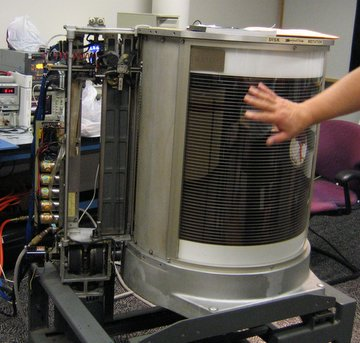
\includegraphics[scale=0.4, angle=0, trim=0 0 0 0]{images/IBM_350.jpg}
        \captionsetup{labelformat=empty,labelsep=none}
        \transparent{0.4}%
        \caption[]{\tiny Image (c) wikipedia.org - Image used solely for illustration purposes}
    \end{figure}
\end{frame}


\begin{frame}[fragile]
  \frametitle{3.1 Storage devices / media}
    \begin{itemize}
        \item Magnetic storage
        \begin{itemize}
            \item Tapes
            \item Floppy disks
            \begin{itemize}
                \item 8" - 1971 - 80KB
                \item 5.25" - 1976 - 360 KB
                \item 3.5" - 1984 - 1.2 MB / - 1986 - 1.44 MB
            \end{itemize}
            \item Hard disks
            \begin{itemize}
                \item IDE / EIDE, Firewire, PATA, SCSI
                \item SATA, SAS Serial attached SCSI, USB, Thunderbolt
            \end{itemize}
        \end{itemize}
        \item Optical storage
        \begin{itemize}
            \item Compact disks - CD
            \item Digital versatile disk - DVD
            \item Blu-ray disk
        \end{itemize}
        \item Non-volatile memory
        \begin{itemize}
            \item USB flash drive
            \item Solid state drive
            \item Flash memory cards
        \end{itemize}
    \end{itemize}
\end{frame}


\begin{frame}[fragile]
  \frametitle{3.2 Physical- / Logical layers}
  \begin{lstlisting}[basicstyle=\tiny]
	  Physical disks
----------  ----------  ----------
| Disc 1 |  | Disc 2 |  | Disc 3 |
----------  ----------  ----------
     |          |           |
     V          V           V
     Logical hard disk volume
----------------------------------
| ------------------------------ |
| |  P1  |    P2    |    P3    | |
| ------------------------------ |
----------------------------------
      |        |          |
      V        V          V
 --------  ---------- ----------
 |  P1  |  |   P2   | |   P3   |
 --------  ---------- ----------
Volume C:  Volume D:  Volume E:
  \end{lstlisting}
\end{frame}


\begin{frame}[fragile]
  \frametitle{3.3 ATA Disks }
    \begin{itemize}
        \item ATA-3: Hard disk password
        \item ATA-4: HPA - Host Protected Area
        \begin{itemize}
            \item Vendor area - benefit system vendors
            \item Recovery data. persistent data
            \item Controlled by firmware not OS
            \item \texttt{READ\_NATIVE\_MAX\_ADDRESS}
        \end{itemize}
        \item ATA-6: DCO - Device Configuration Overlay
        \begin{itemize}
            \item Benefit system vendors
            \item Control reported capacity and disk features
            \item Use disk from different manufacturers
            \item Use disk with different number of sectors
            \item[] $\to$ Makes disks looking uniq
            \item \texttt{DEVICE\_CONFIGURATION\_IDENTIFY}
        \end{itemize}
        \item ATA-7: Serial ATA
    \end{itemize}
\end{frame}


\begin{frame}[fragile]
  \frametitle{3.4 Demo: Hidden Sectors}
    \begin{itemize}
        \item New disk
\begin{lstlisting}[basicstyle=\tiny]
dmesg
    sd 1:0:0:0: [sdb] 3904981168 512-byte logical blocks: (2.00 TB/1.82 TiB)

hdparm -N /dev/sdb
    max sectors   = 3907029168/3907029168, ACCESSIBLE MAX ADDRESS disabled
\end{lstlisting}
        \item Create hidden message
\begin{lstlisting}[basicstyle=\tiny]
echo -n 'MySecret 123456' | dd of=/dev/sdb seek=3500000000

dd if=/bin/dd of=/dev/sdb seek=3500000001
     148+1 records in
     148+1 records out
     76000 bytes (76 kB, 74 KiB) copied, 0,022659 s, 3,4 MB/s
\end{lstlisting}
        \item Create HPA
\begin{lstlisting}[basicstyle=\tiny]
hdparm --yes-i-know-what-i-am-doing -N p3000000000 /dev/sdb
    setting max visible sectors to 3000000000 (permanent)
    max sectors   = 3000000000/3907029168, ACCESSIBLE MAX ADDRESS enabled

Power cycle your device after every ACCESSIBLE MAX ADDRESS
\end{lstlisting}
    \end{itemize}
\end{frame}


\begin{frame}[fragile]
  \frametitle{3.4 Demo: Hidden Sectors}
    \begin{itemize}
        \item Create partition and format
\begin{lstlisting}[basicstyle=\tiny]
dmesg
    sd 1:0:0:0: [sdb] 3000000000 512-byte logical blocks: (1.54 TB/1.40 TiB)

fdisk /dev/sdb
    primary
    2048
    2999999999

mkfs.ntfs -L CIRCL.DFIR -f /dev/sdb1
    Creating NTFS volume structures.
    mkntfs completed successfully. Have a nice day.
\end{lstlisting}
        \item Investigate disk layout
\begin{lstlisting}[basicstyle=\tiny]
fdisk -l /dev/sdb
    Device     Boot Start        End    Sectors  Size Id Type
    /dev/sdb1        2048 2999999999 2999997952  1,4T  7 HPFS/NTFS/exFAT
\end{lstlisting}
        \item Investigate last accessible sector
\begin{lstlisting}[basicstyle=\tiny]
dd if=/dev/sdb skip=2999999999 status=none| xxd
    00000000: eb52 904e 5446 5320 2020 2000 0208 0000  .R.NTFS    .....
      .......
    000001f0: 0000 0000 0000 0000 0000 0000 0000 55aa  ..............U.
\end{lstlisting}
    \end{itemize}
\end{frame}


\begin{frame}[fragile]
  \frametitle{3.4 Demo: Hidden Sectors}
    \begin{itemize}
        \item Try to access hidden message
\begin{lstlisting}[basicstyle=\tiny]
dd if=/dev/sdb skip=3500000000 count=1 | xxd
    dd: /dev/sdb: cannot skip: Invalid argument
    0+0 records in
\end{lstlisting}
        \item Resize HPA
\begin{lstlisting}[basicstyle=\tiny]
hdparm -N /dev/sdb
    max sectors   = 3000000000/3907029168, ACCESSIBLE MAX ADDRESS enabled

hdparm --yes-i-know-what-i-am-doing -N p3900000000 /dev/sdb
    max sectors   = 3900000000/3907029168, ACCESSIBLE MAX ADDRESS enabled

Power cycle your device after every ACCESSIBLE MAX ADDRESS
\end{lstlisting}
        \item Investigate disk layout and last sector
\begin{lstlisting}[basicstyle=\tiny]
fdisk -l /dev/sdb
    Device     Boot Start        End    Sectors  Size Id Type
    /dev/sdb1        2048 2999999999 2999997952  1,4T  7 HPFS/NTFS/exFAT

dd if=/dev/sdb skip=2999999999 status=none | xxd | less
dd if=/dev/sdb skip=3899999999 status=none | xxd | less
\end{lstlisting}
    \end{itemize}
\end{frame}


\begin{frame}[fragile]
  \frametitle{3.4 Demo: Hidden Sectors}
    \begin{itemize}
        \item Recover hidden message
\begin{lstlisting}[basicstyle=\tiny]
dd if=/dev/sdb skip=3500000000 count=1 status=none
    00000000: 4d79 5365 6372 6574 2031 3233 3435 3600  MySecret 123456.
\end{lstlisting}
	\item Recover hidden \texttt{dd} command
\begin{lstlisting}[basicstyle=\tiny]
dd if=/dev/sdb skip=$(( 3500000001*512 )) count=76000 bs=1 of=dd.exe

md5sum dd.exe
    36a70f825b8b71a3d9ba3ac9c5800683

md5sum /bin/dd
    36a70f825b8b71a3d9ba3ac9c5800683
\end{lstlisting}
        \item Feeback: kaplan(at)cert.at
\begin{lstlisting}[basicstyle=\tiny]
    https://www.schneier.com/blog/archives/2014/02/swap_nsa_exploi.html
    https://en.wikipedia.org/wiki/Host_protected_area
\end{lstlisting}
        \item How it works
\begin{lstlisting}[basicstyle=\tiny]
    IDENTIFY DEVICE
    SET MAX ADDRESS
    READ NATIVE MAX ADDRESS
    --> HPA aware software (like the BIOS)
\end{lstlisting}
    \end{itemize}
\end{frame}


\begin{frame}[fragile]
  \frametitle{3.5 Other Hidden Sectors}
    \begin{itemize}
        \item Service area, negative sectors
        \begin{itemize}
            \item Firmware
            \item Bad sectors
            \item ATA passwords
            \item[] \texttt{hdparm --security-unlock "myPassWD" /dev/sdb}
            \item SMART data
	    \item[]
        \end{itemize}
        \item Self-Monitoring, Analysis and Reporting Technology - SMART
        \begin{itemize}
            \item[] \texttt{apt install smartmontools}
            \item[] \texttt{smartctl -x /dev/sdb | less}
\begin{lstlisting}[basicstyle=\tiny]
.....
SMART Attributes Data Structure revision number: 16
Vendor Specific SMART Attributes with Thresholds:
ID# ATTRIBUTE_NAME          FLAGS    VALUE WORST THRESH FAIL RAW_VALUE
  1 Raw_Read_Error_Rate     POSR-K   200   200   051    -    0
  3 Spin_Up_Time            POS--K   234   233   021    -    3258
  4 Start_Stop_Count        -O--CK   100   100   000    -    679
  5 Reallocated_Sector_Ct   PO--CK   200   200   140    -    0
  7 Seek_Error_Rate         -OSR-K   200   200   000    -    0
  9 Power_On_Hours          -O--CK   095   095   000    -    3802
  .....
\end{lstlisting}
        \end{itemize}
    \end{itemize}
\end{frame}


\begin{frame}[fragile]
  \frametitle{3.6 Collecting information from devices}
    \begin{itemize}
        \item[] \texttt{hdparm -I /dev/sdb}
\begin{lstlisting}[basicstyle=\tiny]
ATA device, with non-removable media
        Model Number:       WDC WD20NPVT-00Z2TT0                    
        Serial Number:      WD-WX11A9269540
        Firmware Revision:  01.01A01
        Transport:          Serial, SATA 1.0a, SATA Rev 2.6, SATA Rev 3.0
Standards:
        Supported: 8 7 6 5 
        Likely used: 8
	.....
Security: 
        Master password revision code = 65534    supported
        not     enabled
        not     locked
        not     frozen
        not     expired: security count
        374min for SECURITY ERASE UNIT.
\end{lstlisting}
        \item[] \texttt{hdparm -I /dev/sda}
\begin{lstlisting}[basicstyle=\tiny]
...
Commands/features:
        Enabled Supported:
        ...
           *    Data Set Management TRIM supported (limit 8 blocks)
           *    Deterministic read ZEROs after TRIM
\end{lstlisting}
    \end{itemize}
\end{frame}














\begin{frame}[fragile]
  \frametitle{3.7 How is the device connected}
    \begin{itemize}
        \item Most relevant data with: \texttt{dmesg}
\begin{lstlisting}[basicstyle=\tiny]
dmesg -T
    .....
    [Mi Aug  1 13:06:11 2018] usb-storage 1-1:1.0: USB Mass Storage device detected
    [Mi Aug  1 13:06:11 2018] scsi host1: usb-storage 1-1:1.0
    [Mi Aug  1 13:06:13 2018] scsi 1:0:0:0: Direct-Access USB Flash DISK
    [Mi Aug  1 13:06:13 2018] sd 1:0:0:0: Attached scsi generic sg1 type 0
    [Mi Aug  1 13:06:13 2018] sd 1:0:0:0: [sdb] 15826944 512-byte logical blocks
\end{lstlisting}
        \item Enumerate host hardware
\begin{lstlisting}[basicstyle=\tiny]
lshw | less
    .....

lshw -businfo -class storage
    Bus info          Device           Class          Description
    =============================================================
    pci@0000:04:00.0                   storage        Samsung Electronics Co Ltd
    usb@2:3           scsi0            storage        
    usb@1:1           scsi1            storage

lshw -businfo -class disk
    Bus info          Device           Class          Description
    =============================================================
    scsi@0:0.0.0      /dev/sda         disk           SD/MMC CRW
                      /dev/sda         disk
    scsi@1:0.0.0      /dev/sdb         disk           2TB 2000FYYZ-01UL1B2
\end{lstlisting}
    \end{itemize}
\end{frame}


\begin{frame}[fragile]
  \frametitle{3.7 How is the device connected}
    \begin{itemize}
        \item Enumerate PCI bus
\begin{lstlisting}[basicstyle=\tiny]
lspci -d ::0106                      # List SATA controller

lspci -d ::0108                      # List NVME controller
    04:00.0 Non-Volatile memory controller: Samsung Electronics Co Ltd Device a808

lspci -d ::0C03                      # List USB, FW, ... controller
    00:14.0 USB controller: Intel Corporation Sunrise Point-LP USB 3.0 xHCI Controller (rev 21)
    3b:00.0 USB controller: Intel Corporation JHL6540 Thunderbolt 3 USB Controller (C step) [Alpine Ridge 4C 2016] (rev 02)
    3e:00.0 USB controller: Fresco Logic FL1100 USB 3.0 Host Controller (rev 10)
    40:00.0 USB controller: Fresco Logic FL1100 USB 3.0 Host Controller (rev 10)
\end{lstlisting}
        \item Enumerate block devices
\begin{lstlisting}[basicstyle=\tiny]
lsscsi -v

lsblk /dev/sdb
    NAME   MAJ:MIN RM  SIZE RO TYPE MOUNTPOINT
    sdb      8:16   0  1,8T  0 disk
     sdb1   8:17   0  1,8T  0 part /media/mich/031F0F30642CBB8B

lsblk -pd -o TRAN,NAME,SERIAL,VENDOR,MODEL,REV,WWN,SIZE,HCTL,SUBSYSTEMS /dev/sdb
    TRAN NAME     SERIAL          VENDOR   MODEL
    usb  /dev/sdb WD-WMC1P0H10ZEX WT055 WD 2000FYYZ-01UL1B2
             REV WWN                 SIZE HCTL       SUBSYSTEMS
            01.0 0x50014ee05979e023  1,8T 1:0:0:0    block:scsi:usb:pci
\end{lstlisting}
    \end{itemize}
\end{frame}


\begin{frame}[fragile]
	\frametitle{3.8 USB enumeration}
    \begin{itemize}
        \item List attached USB device
        \begin{itemize}
            \item USB bus
            \item Device address
            \item Vendor ID
            \item Product ID
            \item Product details
            \item[] ...
        \end{itemize}
        \item[] \texttt{lsusb}
\begin{lstlisting}[basicstyle=\tiny]
Bus 004 Device 001: ID 1d6b:0003 Linux Foundation 3.0 root hub
Bus 003 Device 001: ID 1d6b:0002 Linux Foundation 2.0 root hub
Bus 002 Device 002: ID 0bda:0328 Realtek Semiconductor Corp. 
Bus 002 Device 003: ID 1b1c:1a0e Corsair 
Bus 002 Device 004: ID 0951:162b Kingston Technology 
Bus 002 Device 001: ID 1d6b:0003 Linux Foundation 3.0 root hub
Bus 001 Device 004: ID 06cb:009a Synaptics, Inc. 
Bus 001 Device 003: ID 04f2:b61e Chicony Electronics Co., Ltd 
Bus 001 Device 001: ID 1d6b:0002 Linux Foundation 2.0 root hub
\end{lstlisting}
    \end{itemize}
\end{frame}


\begin{frame}[fragile]
	\frametitle{3.8 USB enumeration}
    \begin{itemize}
        \item[] \texttt{lsusb -t}
\begin{lstlisting}[basicstyle=\tiny]
/:  Bus 04.Port 1: Dev 1, Class=root_hub, Driver=xhci_hcd/2p, 10000M
/:  Bus 03.Port 1: Dev 1, Class=root_hub, Driver=xhci_hcd/2p, 480M
/:  Bus 02.Port 1: Dev 1, Class=root_hub, Driver=xhci_hcd/6p, 5000M
    |__ Port 1: Dev 4, If 0, Class=Mass Storage, Driver=usb-storage, 5000M
    |__ Port 2: Dev 3, If 0, Class=Mass Storage, Driver=uas, 5000M
    |__ Port 3: Dev 2, If 0, Class=Mass Storage, Driver=usb-storage, 5000M
/:  Bus 01.Port 1: Dev 1, Class=root_hub, Driver=xhci_hcd/12p, 480M
    |__ Port 8: Dev 3, If 1, Class=Video, Driver=uvcvideo, 480M
    |__ Port 8: Dev 3, If 0, Class=Video, Driver=uvcvideo, 480M
    |__ Port 9: Dev 4, If 0, Class=Vendor Specific Class, Driver=, 12M
\end{lstlisting}
        \item[] \texttt{lsusb  -v -d 0951:162b`}
\begin{lstlisting}[basicstyle=\tiny]
...
    Interface Descriptor:
      bLength                 9
      bDescriptorType         4
      bInterfaceNumber        0
      bAlternateSetting       0
      bNumEndpoints           2
      bInterfaceClass         8 Mass Storage
      bInterfaceSubClass      6 SCSI
      bInterfaceProtocol     80 Bulk-Only
...
\end{lstlisting}
    \end{itemize}
\end{frame}


\begin{frame}[fragile]
    \frametitle{3. usbmon \& wireshark}
	\frametitle{3.9 USB Interface monitoring}
    \begin{figure}
        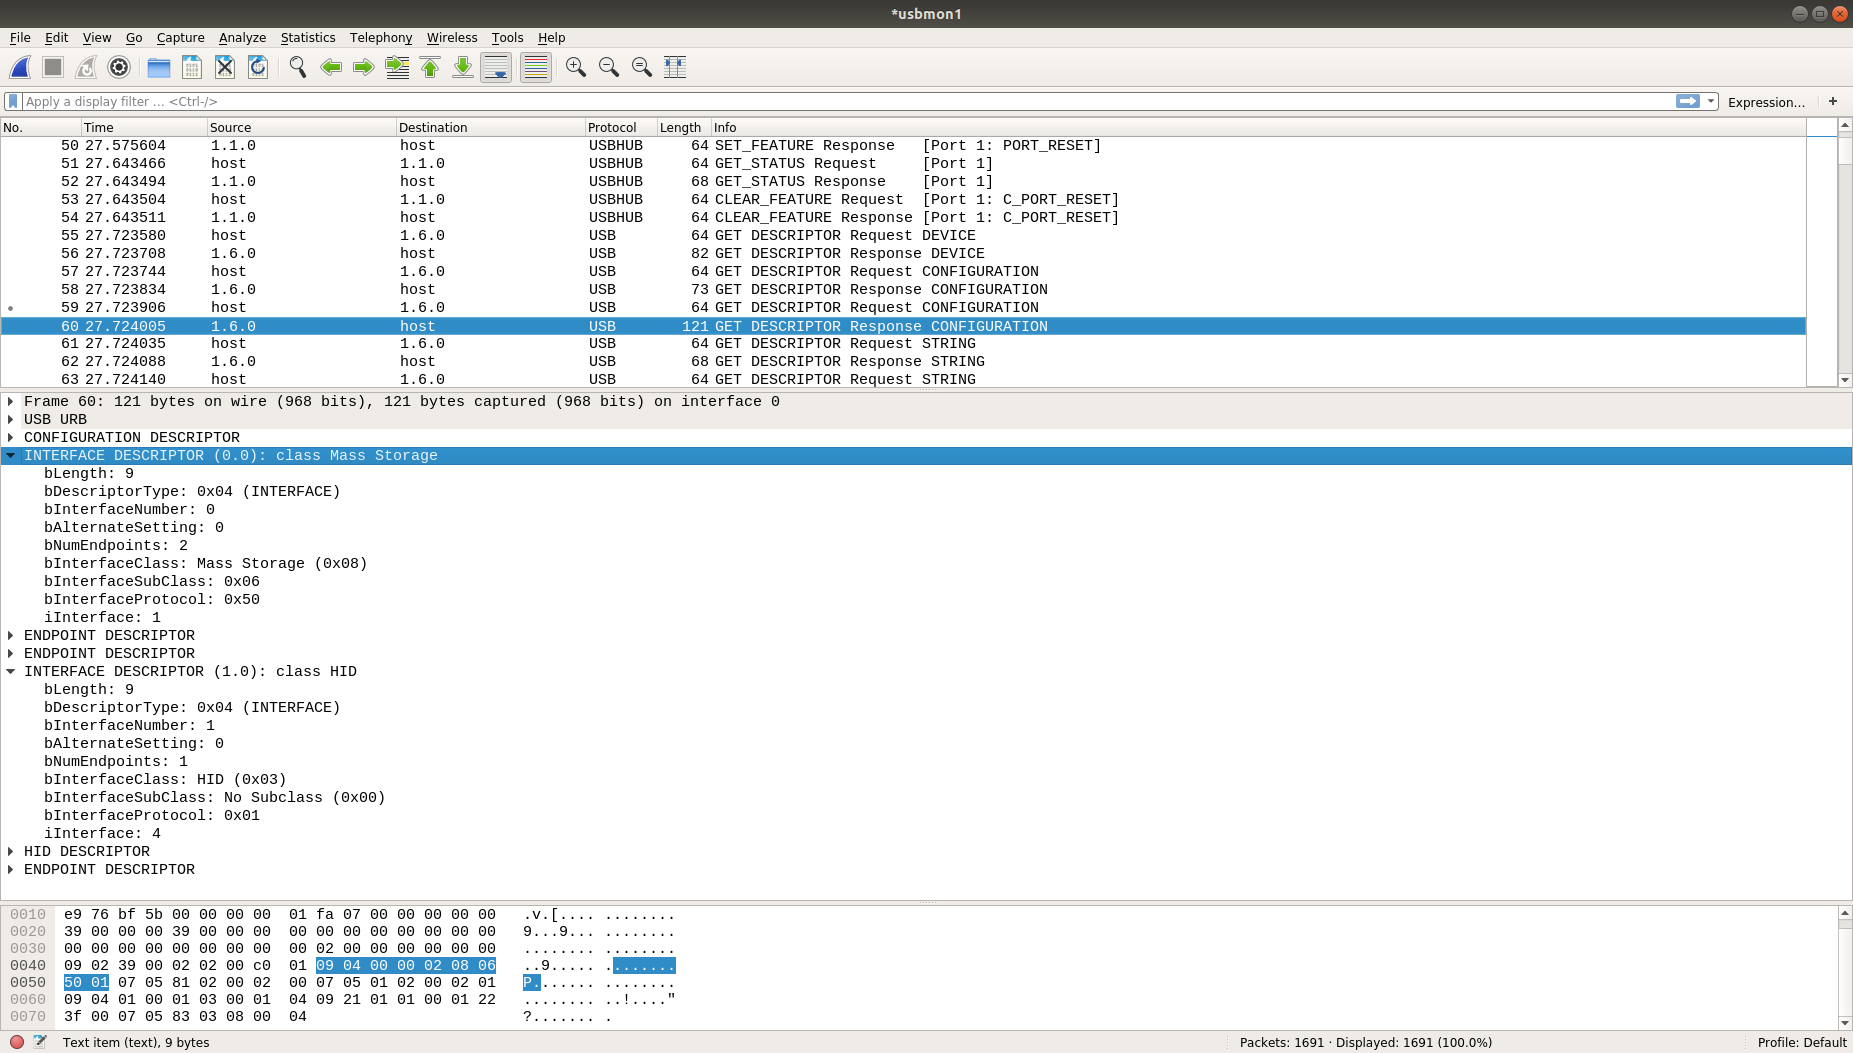
\includegraphics[scale=0.18, angle=0, trim=0 0 0 0]{images/usbmon.png}\llap{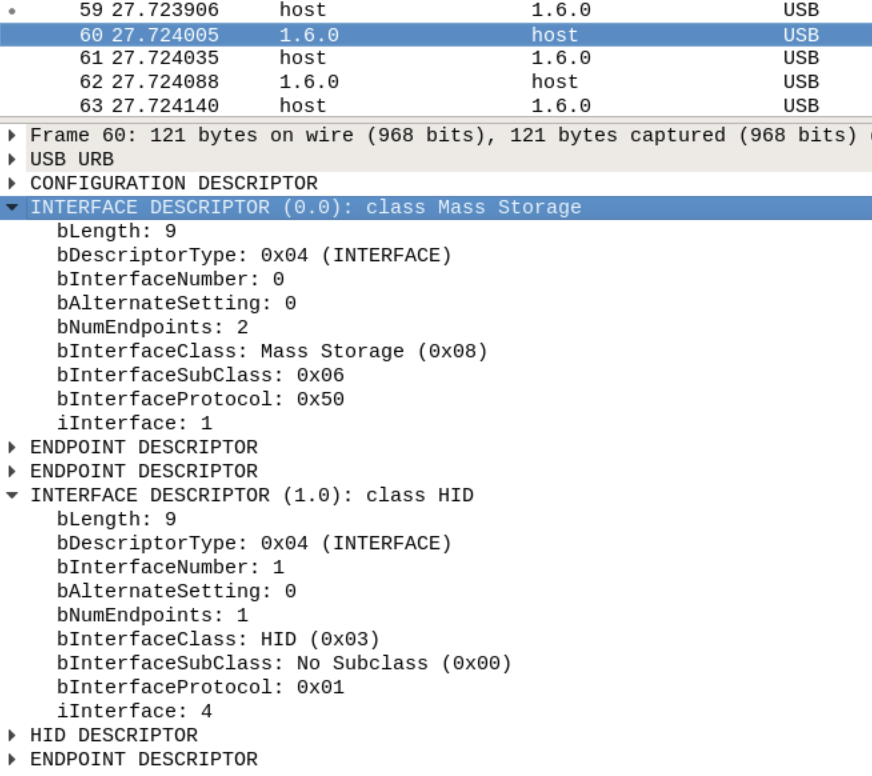
\includegraphics[scale=0.27, trim = 0px 0px 0px 0px, angle=-5]{images/usbmon2.png}}
        % 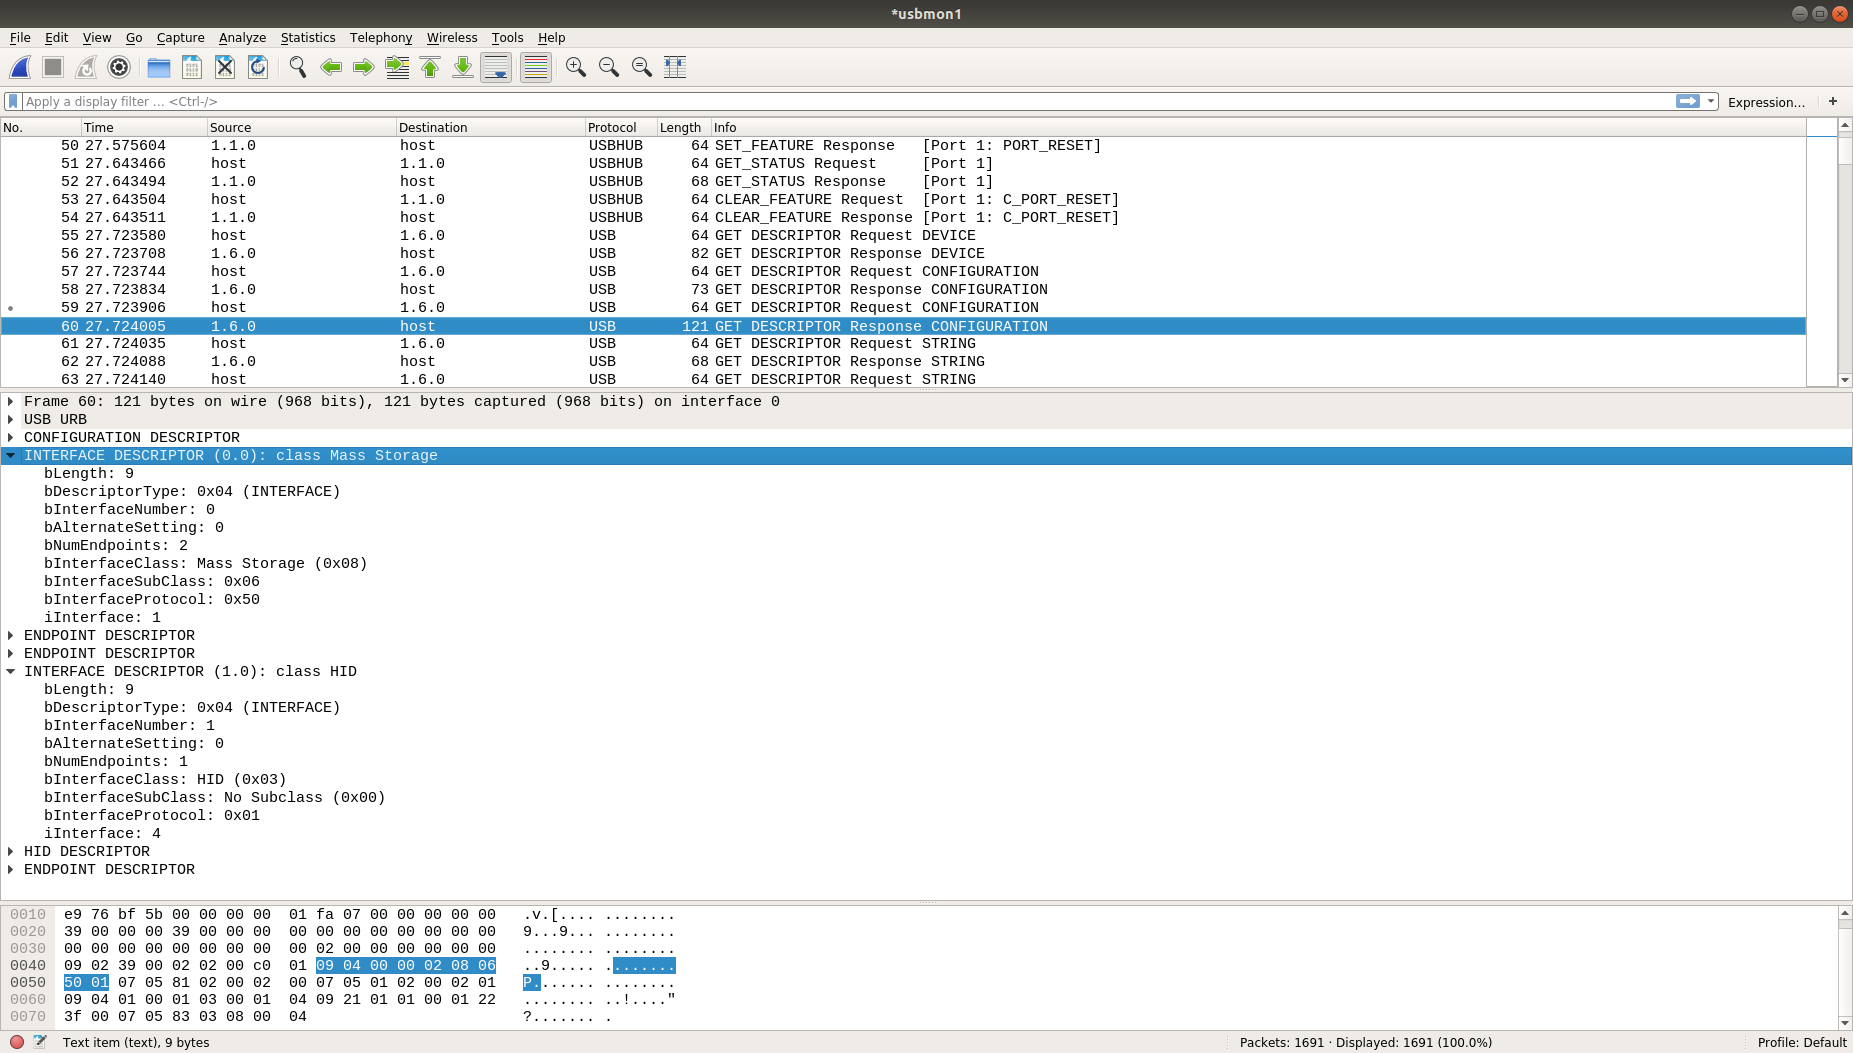
\includegraphics[scale=0.18, angle=0, trim=0 0 0 0]{images/usbmon.png}\llap{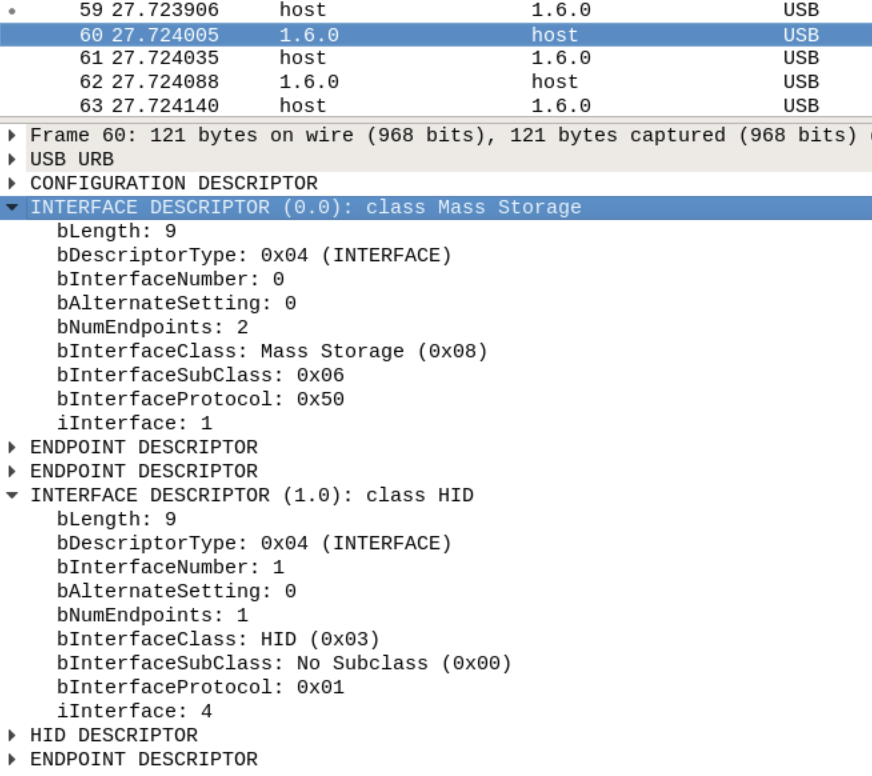
\includegraphics[height=5cm]{images/usbmon2.png}}
        \captionsetup{labelformat=empty,labelsep=none}
    \end{figure}
\end{frame}




% DO NOT COMPILE THIS FILE DIRECTLY!
% This is included by the other .tex files.


\begin{frame}
    
\includegraphics[scale=0.3]{images/logo-circl-Forensics.png}
    \begin{itemize}
        \item[]
        \item[]
        \item[] 4. Disk Cloning / Disk Imaging
    \end{itemize}
\end{frame}


\begin{frame}[fragile]
  \frametitle{4.1 Disk cloning - imaging}
    \begin{itemize}
        \item Clone disk-2-disk
        \begin{itemize}
            \item Different sizes
            \item Wipe target disk!
        \end{itemize}
        \item Clone disk-2-image
        \begin{itemize}
            \item Clear boundaries
            \item One big file
            \item Break file into chunks
        \end{itemize}
        \item Image file format
        \begin{itemize}
            \item RAW
            \item AFF (Advanced Forensic Format)
            \item EWF (Expert Witness Format)
            \item Please no 3rd party formats
        \end{itemize}
        \item Write-Blockers
        \begin{itemize}
            \item Hardware
        \end{itemize}
    \end{itemize}
\end{frame}


\begin{frame}[fragile]
  \frametitle{4.2 Connecting devices}
    \begin{itemize}
        \item \texttt{udev} 
\begin{lstlisting}[basicstyle=\tiny]
udevadm info /dev/sda                 # userspace /dev
udevadm monitor
\end{lstlisting}
        \item \texttt{/dev/}
\begin{lstlisting}[basicstyle=\tiny]
/dev/sd*               # SCSI, SATA
/dev/hd*               # IDE. EIDE
/dev/md*               # RAID
/dev/nvme*n*           # NVME devices

/dev/sda1              # Partition 1 on disk 1
/dev/sda2              # Partition 2 on disk 1
...
\end{lstlisting}
        \item Block Devices
        \begin{itemize}
            \item Attaching
            \item Mounting
        \end{itemize}
    \end{itemize}
\end{frame}


\begin{frame}[fragile]
  \frametitle{4.2 Read partition table}
    \begin{itemize}
        \item \texttt{dmesg} 
\begin{lstlisting}[basicstyle=\tiny]
[106834.127269] sd 6:0:0:0: Attached scsi generic sg1 type 0
[106834.127503] sd 6:0:0:0: [sdb] 15826944 512-byte logical blocks: (8.10 GB/7.54 GiB)
[106834.130380] sd 6:0:0:0: [sdb] Write Protect is off
\end{lstlisting}
        \item \texttt{fdisk -l circl-dfir.dd}
\begin{lstlisting}[basicstyle=\tiny]
Disk circl-dfir.dd: 1536 MB, 1536000000 bytes
4 heads, 7 sectors/track, 107142 cylinders, total 3000000 sectors
Units = sectors of 1 * 512 = 512 bytes
Sector size (logical/physical): 512 bytes / 512 bytes
I/O size (minimum/optimal): 512 bytes / 512 bytes
Disk identifier: 0x8f7e6594

        Device Boot      Start         End      Blocks   Id  System
circl-dfir.dd1            2048     3000000     1498976+   7  HPFS/NTFS/exFAT
\end{lstlisting}
        \item Exercise: Analyze output. Why \texttt{1498976}? $\to$ Conclusions?
    \end{itemize}
\begin{lstlisting}[basicstyle=\tiny]
End:     echo $(( 3000000 * 512 ))                  --> 1536 MB, 1536000000 bytes 
         echo $(( 3000000 * 512 / 1024 / 1024 ))    --> 1464

1498976: echo $(( 1498976 * 2 ))                    --> 2997952
\end{lstlisting}
\end{frame}


\begin{frame}[fragile]
  \frametitle{4.2 Mounting}
    \begin{itemize}
        \item \texttt{mount} 
\begin{lstlisting}[basicstyle=\tiny]
mkdir /mnt/ntfs                             # Create mount point
mount /dev/sdb1 /mnt/ntfs                   # Mounting

mount -o ro,remount /dev/sdb1 /mnt/ntfs     # Re-mounting

umount /mnt/ntfs                            # Un-mounting
umount /dev/sdb1                            # Also un-mounting


# Mounting readonly, no journaling, no executable
mount -o ro,noload,noexec /dev/sdb1 /mnt/ntfs
mount -o ro,noload,noexec,remount /dev/sdb1 /mnt/ntfs


# Mounting with offset. mounting from image files
mount -o ro,noload,noexec,offset=$((512*2048)) circl-dfir.dd /mnt/ntfs


# Mounting NTFS file systems
mount -o ro,noload,noexec,offset=$((512*2048)),
      show_sys_files,streams_interface=windows circl-dfir.dd /mnt/ntfs

\end{lstlisting}
    \end{itemize}
\end{frame}


\begin{frame}[fragile]
  \frametitle{4.3 dd - disk imaging rudimentary}
    \begin{itemize}
        \item[] Copy files from: \texttt{/mnt/ntfs/dd/}
\begin{lstlisting}[basicstyle=\tiny]
$ dd if=img_1.txt of=out_1.txt bs=512

     <input file>      <output file> <block size>
                                      (default)
3+0 records in
3+0 records out
1536 bytes (1.5 kB) copied, 0.000126 s, 12.2 MB/s

$ ll
-rw-rw-r-- 1 hamm hamm 1536 May 16 11:20 img_1.txt
-rw-rw-r-- 1 hamm hamm 1536 May 16 11:16 out_1.txt



$ dd if=img_2.txt of=out_2.txt bs=512
3+1 records in
3+1 records out
1591 bytes (1.6 kB) copied, 0.00016048 s, 9.9 MB/s

$ ll
-rw-rw-r-- 1 hamm hamm 1591 May 16 11:20 img_2.txt
-rw-rw-r-- 1 hamm hamm 1591 May 16 11:26 out_2.txt
\end{lstlisting}
    \end{itemize}
\end{frame}


\begin{frame}[fragile]
  \frametitle{4.3 dd - disk imaging rudimentary}
    \begin{itemize}
        \item[] Demo: \texttt{skip} and \texttt{count} options
\begin{lstlisting}[basicstyle=\tiny]
dd if=img_3.txt bs=512 skip=0 count=1 status=none | less
dd if=img_3.txt bs=512 skip=1 count=1 status=none | less
dd if=img_3.txt bs=512 skip=2 count=1 status=none | less
\end{lstlisting}
        \item[] Exercise: Find the secret password behind sector 3
        \item[] Exercise: Play with \texttt{bs, skip} and \texttt{count} options
\begin{lstlisting}[basicstyle=\tiny]
dd if=img_3.txt bs=1 skip=$((512*3)) count=16 status=none
dd if=img_3.txt bs=16 skip=$((32*3)) count=1 status=none
\end{lstlisting}
        \item[] Exercise: \texttt{dd | xxd | less}
\begin{lstlisting}[basicstyle=\tiny]
dd if=img_3.txt bs=512 skip=3 count=1 status=none | xxd | less
	0+1 records in
	0+1 records out
	55 bytes (55 B) copied, 5.04e-05 s, 1.1 MB/s

0000000: 4f76 6572 6865 6164 2031 3233 3435 3637  Overhead 1234567
0000010: 3839 3020 204d 6573 7361 6765 2d31 2020  890  Message-1  
0000020: 3039 3837 3635 3433 3231 2020 2020 2020  0987654321      
0000030: 2020 2020 2020 20
\end{lstlisting}
    \end{itemize}
\end{frame}


\begin{frame}[fragile]
  \frametitle{4.3 dd - disk imaging rudimentary}
    \begin{itemize}
        \item[] Demo: Continue an interrupted imaging process
\begin{lstlisting}[basicstyle=\tiny]
dd if=img_2.txt of=broken.raw bs=512 skip=0 count=2 status=none

ll  img_2.txt  ..... 1591 Aug 13 14:40 img_2.txt*
ll broken.raw  ..... 1024 Aug 13 15:05 broken.raw

dd if=img_2.txt of=broken.raw bs=512 skip=2 seek=2 status=none

md5sum  img_2.txt f319b1cc9d424a923a8c83c3e67185f1
md5sum broken.raw f319b1cc9d424a923a8c83c3e67185f1
\end{lstlisting}
        \item[] Error handling: Bad blocks
\begin{lstlisting}[basicstyle=\tiny]
$ dd if=img_3.txt of=out_3.txt bs=512 conv=noerror,sync
\end{lstlisting}
        \item[] Demo: Progress
        \begin{itemize}
            \item[] Option: \texttt{status=progress}
            \item[] Signaling: \texttt{'\&' and 'kill -10'}
        \end{itemize}
    \end{itemize}
\end{frame}


\begin{frame}[fragile]
  \frametitle{4.4 Disk acquisition}
    \begin{itemize}
        \item Forensic features
        \begin{itemize}
            \item Progress monitoring
            \item Error handling \& logging
            \item Meta data
            \item Splitting output files \& support of forensic formats
            \item Cryptographic hashing \& verification checking
        \end{itemize}
        \item Example: hashing
        \begin{itemize}
            \item[] \texttt{md5sum circl-dfir.dd} $\to$ \texttt{bd80672b9d1bef2f35b6e902f389e83}
            \item[] \texttt{sha1sum circl-dfir.dd} $\to$ \texttt{e5ffc7233a..........7e53b9f783}
        \end{itemize}
        \item Tools
        \begin{itemize}
            \item dd
            \item ddrescue, gddrescue, dd\_rescue
            \item dc3dd - Department of Defense Cyber Crime Center
            \item dcfldd - Defense Computer Forensic Labs
	    \item rdd-copy, netcat, socat, ssh
            \item Guymager
        \end{itemize}
    \end{itemize}
\end{frame}


\begin{frame}[fragile]
  \frametitle{4.5 Exercise: dc3dd}
  \begin{lstlisting}[basicstyle=\tiny]
dc3dd if=/mnt/ntfs/carving/deleted.dd                   # Input file
      log=usb.log  -/                                   # Logging
      hash=md5 hash=sha1  -/                            # Hashing
      ofsz=$((8*1024*1024)) ofs=usb.raw.000             # Chunk files of 8MB


ls -l


cat usb.log


cat usb.raw.00* | md5sum                                # Verify hashes
cat usb.raw.00* | sha1sum


dc3dd wipe=/dev/sdx                                     # Wipe a drive
  \end{lstlisting}
\end{frame}


\begin{frame}[fragile]
  \frametitle{4.6 SuashFS as forensic container}
    \begin{itemize}
        \item Embedded systems
        \item Read only file system
        \item Supports very large files
        \item Adding files possible
        \item Deleting, modifying files not possible
        \item Compressed
	\item[] $\to$ Real case: 3*1TB disks stored in 293GB container
	\item Bruce Nikkel: \url{http://digitalforensics.ch/sfsimage/}
    \end{itemize}
  \begin{lstlisting}[basicstyle=\tiny]
mksquashfs circl-dfir.dd case_123.sfs
mksquashfs analysis.txt case_123.sfs
unsquashfs -ll case_123.sfs
.....
mksquashfs analysis.txt case_123.sfs
.....
sudo mount case_123.sfs /mnt/
  \end{lstlisting}
\end{frame}


\begin{frame}[fragile]
  \frametitle{4.7 Exercise: Modify data on RO mounted device}
  \begin{lstlisting}[basicstyle=\tiny]
mount
mount -o ro,remount /media/michael/7515-6AA5/
mount


Demo: Modify Document

strings -td /dev/sdb1
    .....
    299106 Hello World!
    .....

echo $((299106/512))
    584

dd if=/dev/sdb1 bs=512 skip=584 count=1 of=584.raw
ll
hexer 584.raw

dd of=/dev/sdb1 bs=512 seek=584 count=1 if=584.raw
mount


Demo: Review Document
  
  
  \end{lstlisting}
\end{frame}


\begin{frame}
    \frametitle{4.7 Exercise: RO Countermeasures}
    \begin{itemize}
        \item Try on board methods:
        \begin{itemize}
            \item[]
            \begin{itemize}
                \item \texttt{hdparm -r1 /dev/sdb}
                \item \texttt{blockdev --setro /dev/sdb}
                \item \texttt{udev} rules
                \item[] $\to$ Attack on block device still possible
            \end{itemize}
        \end{itemize}
        \item Try Forensics Linux Distributions:
        \begin{itemize}
            \item Live Kali 2018\_4 in forensic mode
            \item SANS SIFT Workstation 3.0
            \item DEFT X 8.2 DFIR Toolkit
            \begin{itemize}
                \item Some distributions do not auto mount
                \item[] $\to$ Attack on block device still possible
            \end{itemize}
        \end{itemize}
\item Kernel Patch: Linux write blocker (not tested)
        \begin{itemize}
                \item[] $\to$ \url{https://github.com/msuhanov/Linux-write-blocker}
        \end{itemize}
        \item Hardware Write Blocker
        \begin{itemize}
            \item[]
            \begin{itemize}
                \item[] $\to$ Effectively block attack
            \end{itemize}
        \end{itemize}
    \end{itemize}
\end{frame}





% DO NOT COMPILE THIS FILE DIRECTLY!
% This is included by the other .tex files.


\begin{frame}
    
\includegraphics[scale=0.3]{images/logo-circl-Forensics.png}
    \begin{itemize}
        \item[]
        \item[]
        \item[] 5. Disk Analysis
    \end{itemize}
\end{frame}


\begin{frame}
  \frametitle{5.1 CHS - Cylinder Head Sector}
    \begin{itemize}
        \item[] Track, Head, Cylinder, Sector, Block, Cluster
    \end{itemize}
    \begin{figure}
        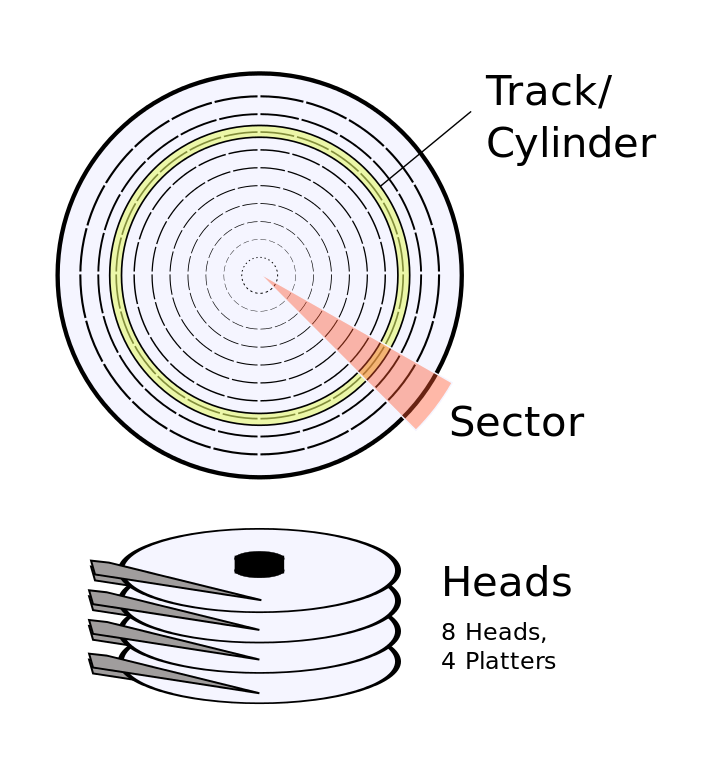
\includegraphics[scale=0.2]{images/chs.png}
        \captionsetup{labelformat=empty,labelsep=none}
        \transparent{0.4}%
        \caption[]{\tiny Image (c) wikipedia.org - Image used solely for illustration purposes}
    \end{figure}
\end{frame}


\begin{frame}[fragile]
  \frametitle{5.2 LBA - Logical Block Addressing}
  \begin{lstlisting}[basicstyle=\tiny\ttfamily]
Logical volume addresses
----------------------------------------------------------------------------
|  0 |  1 |  2 |  3 |  4 |  5 |  6 |  7 |  8 |  9 | 10 | 11 | 12 | 13 | 14 |
----------------------------------------------------------------------------
          |                   |                   |                   |
          |                   |                   |                   |
          -------------------------------------------------------------
   ^      |         0         |         1         |         3         |   ^
   |      -------------------------------------------------------------   |
   |      Logical file system addresses - Clusters                        |
  MBR                                                               Volume slack
          *-------------------*
               2.048 Bytes
          *-----------------------------------------------------------*
                                   6.144 Bytes
  \end{lstlisting}
\end{frame}


\begin{frame}[fragile]
  \frametitle{5.3 Low-Level: Sector Structur}
    \begin{figure}
        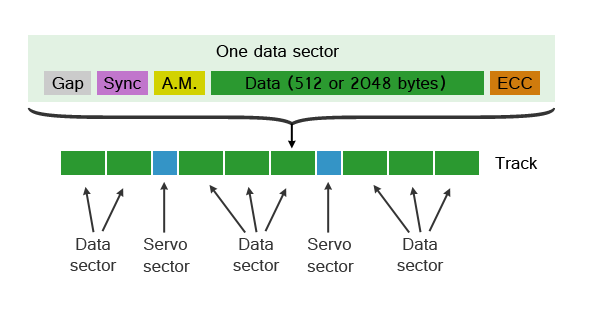
\includegraphics[scale=0.5]{images/sector.png}
        \captionsetup{labelformat=empty,labelsep=none}
        \transparent{0.4}%
        \caption[]{\tiny Image (c) forensicfocus.com - Image used solely for illustration purposes}
    \end{figure}
\end{frame}


\begin{frame}[fragile]
  \frametitle{5.3 Low-Level: Encoding digital data}
        \begin{enumerate}
            \item FM - Frequency Modulation
\begin{lstlisting}[basicstyle=\tiny]
        -----       -----       -----       -----   Clock
 |     |     |     |     |     |     |     |
  -----       -----       -----       -----
 .  0  .  0  .  0  .  0  .  0  .  0  .  0  .  0  .
 .     .     .     .     .     .     .     .     .
        --    -----       --    --    --    -----   Data + Clock
 |     |  |  |     |     |  |  |  |  |  |  |
  -----    --       -----    --    --    --
    0     1     0     0     1     1     1     0
\end{lstlisting}
	    \item MFM - Modified Frequency Modulation (Double Density)
\begin{lstlisting}[basicstyle=\tiny]
        -----       -----       -----       -----   Clock
 |     |     |     |     |     |     |     |
  -----       -----       -----       -----
 .  0  .  0  .  0  .  0  .  0  .  0  .  0  .  0  .
 .     .     .     .     .     .     .     .     .
           -- -----          -- --       -- -----   Data - Clock
 |        |        |        |     |     |    
  ----- --          ----- --       -- --    
    0     1     0     0     1     1     1     0
\end{lstlisting}
	    \item RLL - Run Length Limited
	    \item PRML, EPRML - Extended Partial Response Maximun Likehood
        \end{enumerate}
\end{frame}



\begin{frame}[fragile]
  \frametitle{5.4 MBR - Master Boot Record}
  \begin{lstlisting}[basicstyle=\tiny]
# dd if=/dev/sdc bs=512 count=1 skip=0 |xxd

0000000: fab8 0010 8ed0 bc00 b0b8 0000 8ed8 8ec0  ................
0000016: fbbe 007c bf00 06b9 0002 f3a4 ea21 0600  ...|.........!..
0000032: 00be be07 3804 750b 83c6 1081 fefe 0775  ....8.u........u
0000048: f3eb 16b4 02b0 01bb 007c b280 8a74 018b  .........|...t..
0000064: 4c02 cd13 ea00 7c00 00eb fe00 0000 0000  L.....|.........
0000080: 0000 0000 0000 0000 0000 0000 0000 0000  ................
0000096: 0000 0000 0000 0000 0000 0000 0000 0000  ................
...
...
0000432: 0000 0000 0000 0000 9af0 0200 0000 0020  ............... 
0000448: 2100 0b1b 0299 0008 0000 0080 2500 00a8  !...........%...
0000464: 01a8 071a b327 0058 2900 00c0 5d00 001a  .....'.X)...]...
0000480: b427 076c dad2 0018 8700 00c0 6800 0000  .'.l........h...
0000496: 0000 0000 0000 0000 0000 0000 0000 55aa  ..............U.



000 - 439       0x000 - 0x1B7    Boot code
440 - 443       0x1B8 - 0x1BB    Disc signature
444 - 445       0x1BC - 0x1BD    Reserved
446 - 509       0x1BE - 0x1FD    Partitiontable
510 - 511       0x1FE - 0x1FF    0x55 0xAA
  \end{lstlisting}
\end{frame}


\begin{frame}[fragile]
  \frametitle{5.5 MBR - DOS Partition Table}
  \begin{lstlisting}[basicstyle=\tiny,escapechar=\*]
# dd if=/dev/sdc bs=512 count=1 skip=0 |xxd

0000000: fab8 0010 8ed0 bc00 b0b8 0000 8ed8 8ec0  ................
0000016: fbbe 007c bf00 06b9 0002 f3a4 ea21 0600  ...|.........!..
0000032: 00be be07 3804 750b 83c6 1081 fefe 0775  ....8.u........u
0000048: f3eb 16b4 02b0 01bb 007c b280 8a74 018b  .........|...t..
0000064: 4c02 cd13 ea00 7c00 00eb fe00 0000 0000  L.....|.........
0000080: 0000 0000 0000 0000 0000 0000 0000 0000  ................
0000096: 0000 0000 0000 0000 0000 0000 0000 0000  ................
...
...
0000432: 0000 0000 0000 0000 9af0 0200 0000 *\underline{0020}*  ............... 
0000448: 2100 0b1b 0299 0008 0000 0080 2500 *\underline{00a8}*  !...........%...
0000464: 01a8 071a b327 0058 2900 00c0 5d00 *\underline{001a}*  .....'.X)...]...
0000480: b427 076c dad2 0018 8700 00c0 6800 *\underline{0000}*  .'.l........h...
0000496: 0000 0000 0000 0000 0000 0000 0000 55aa  ..............U.



Partitiontable:
  Offset: 0     Size: 1	Value: 0x80     --> Bootable
  Offset: 1     Size: 3	Value:          --> Starting CHS address
  Offset: 4     Size: 1	Value: 0x0b     --> FAT32
                               0x07     --> NTFS
  Offset: 5     Size: 3	Value:          --> Ending CHS address
  Offset: 8     Size: 4 Value:          --> Starting LBA address
  Offset:12     Size: 4 Value:          --> LBA size in sectors

  \end{lstlisting}
\end{frame}


\begin{frame}[fragile]
  \frametitle{5.5 MBR - DOS Partition Table}
  \begin{lstlisting}[basicstyle=\tiny,escapechar=\?]
  0000432: 0000 0000 0000 ?\texttt{0000 9af0}? ?\texttt{0200 0000}? 0020  ............... 
  0000448: 2100 0b1b 0299 ?\underline{0008 0000}? ?\underline{0080 2500}? 00a8  !...........%...
  0000464: 01a8 071a b327 ?\underline{0058 2900}? ?\underline{00c0 5d00}? 001a  .....'.X)...]...
  0000480: b427 076c dad2 ?\underline{0018 8700}? ?\underline{00c0 6800}? 0000  .'.l........h...
  0000496: 0000 0000 0000 ?\underline{0000 0000}? ?\underline{0000 0000}? 55aa  ..............U.

Partitiontable:
  Offset: 0     Size: 1	Value: 0x80     --> Bootable
  Offset: 1     Size: 3	Value:          --> Starting CHS address
  Offset: 4     Size: 1	Value: 0x0b     --> FAT32
                               0x07     --> NTFS
  Offset: 5     Size: 3	Value:          --> Ending CHS address
  Offset: 8     Size: 4 Value:          --> Starting LBA address
  Offset:12     Size: 4 Value:          --> LBA size in sectors
  
Addressable space:
  CHS: echo $((2**8 * 2**6 * 2**10 * 512 / 1024**2))  ==  8192 MByte
  LBA: echo $((2**32 * 512 / 1024**3))                ==  2048 GByte
  \end{lstlisting}
    \begin{itemize}
        \item Exercise: Calculate the size if the partitions
        \begin{enumerate}
            \item Take LBA size
	    \item Apply Little Endian
	    \item Apply sector size
        \end{enumerate}
    \end{itemize}
\end{frame}


\begin{frame}[fragile]
  \frametitle{5.5 MBR - DOS Partition Table}
  \begin{lstlisting}[basicstyle=\tiny,escapechar=\?]
  0000432: 0000 0000 0000 ?\texttt{0000 9af0}? ?\texttt{0200 0000}? 0020  ............... 
  0000448: 2100 0b1b 0299 ?\underline{0008 0000}? ?\underline{0080 2500}? 00a8  !...........%...
  0000464: 01a8 071a b327 ?\underline{0058 2900}? ?\underline{00c0 5d00}? 001a  .....'.X)...]...
  0000480: b427 076c dad2 ?\underline{0018 8700}? ?\underline{00c0 6800}? 0000  .'.l........h...
  0000496: 0000 0000 0000 ?\underline{0000 0000}? ?\underline{0000 0000}? 55aa  ..............U.

  \end{lstlisting}
    \begin{itemize}
        \item Exercise: Calculate the size if the partitions
    \end{itemize}
  \begin{lstlisting}[basicstyle=\tiny]
        LBA size       Little Endian              Sector size
-----------------------------------------------------------------------------
Part1:  0x00802500     0x00258000     2457600     * 512     1258291200   1.2 GB
Part2:  0x00c05d00     0x005dc000     6144000     * 512     3145728000   3.0 GB
Part3:  0x00c06800     0x0068c000     6864896     * 512     3514826752   3.4 GB
  \end{lstlisting}
    \begin{itemize}
        \item Demo:     Change partition type with hexeditor
	\item[] \texttt{fdisk -l /dev/sdb; hexedit /dev/sdb; F2, CTRL+x}
	\item[]
        \item Exercise: Find password in unused space before first partition
    \end{itemize}
\end{frame}


\begin{frame}[fragile]
  \frametitle{5.6 Extended Partition - EBR}
  \begin{lstlisting}[basicstyle=\tiny]
...
0000432: 0000 0000 0000 0000 0000 0000 0000 0020  ............... 
0000448: 2100 0b1b 0299 0008 0000 0080 2500 00a8  !...........%...
0000464: 01a8 071a b327 0058 2900 00c0 5d00 0000  .....'.X)...]...
0000480: 0000 0000 0000 0000 0000 0000 0000 0000  ................
0000496: 0000 0000 0000 0000 0000 0000 0000 55aa  ..............U.


Partition table:
446 - 461       0x1BE - 0x1CD    1th entry - This logical partition
462 - 477       0x1CE - 0x1DD    2nd entry - Empty OR Next EBR - Extended Boot Record
478 - 493       0x1DE - 0x1ED    Unused
494 - 509       0x1EE - 0x1FD    Unused


-----------------------------------------------------------------------------------
| Extended Partition                                                              |
-----------------------------------------------------------------------------------
| EBR | Logical         | Extended partition                                      |
|     | Partition       -----------------------------------------------------------
| --> |                 | EBR | Logical          | Extended partition             |
| ----+---------------> |     |                  ---------------------------------|
|     |                 | --> |                  | EBR | Logical                  |
|     |                 | ----+----------------> |     |                          |
|     |                 |     |                  | --> |                          |
|     |                 |     |                  | 000 |                          |
-----------------------------------------------------------------------------------
  \end{lstlisting}
\end{frame}


\begin{frame}[fragile]
  \frametitle{5.7 GPT - GUID Partition Table}
    \begin{itemize}
        \item BIOS $\to$ UEFI - Unified Extensible Firmware Interface
	\item GUID - Globally Unique Identifier for each partition
	\item[] $\to$ GUID Partition Table
	\item Protective MBR at LBA0
        \begin{itemize}
            \item One single entry covering the entire disk
            \item Partition type 0xEE
	    \item[] if 0xEE unknown $\to$ Not empty $\to$ Not formatted
        \end{itemize}
	\item GPT header at LBA1
	\item GPT entries at LBA2 $\to$ LBA34
	\item GPT entries: 128 Bytes
	\item GPT backup at end of disk
    \end{itemize}
\end{frame}


\begin{frame}[fragile]
  \frametitle{5.7 GPT - GUID Partition Table}
    \begin{figure}
        \caption[]{\tiny Image (c) wikipedia.org - Image used solely for illustration purposes}
	    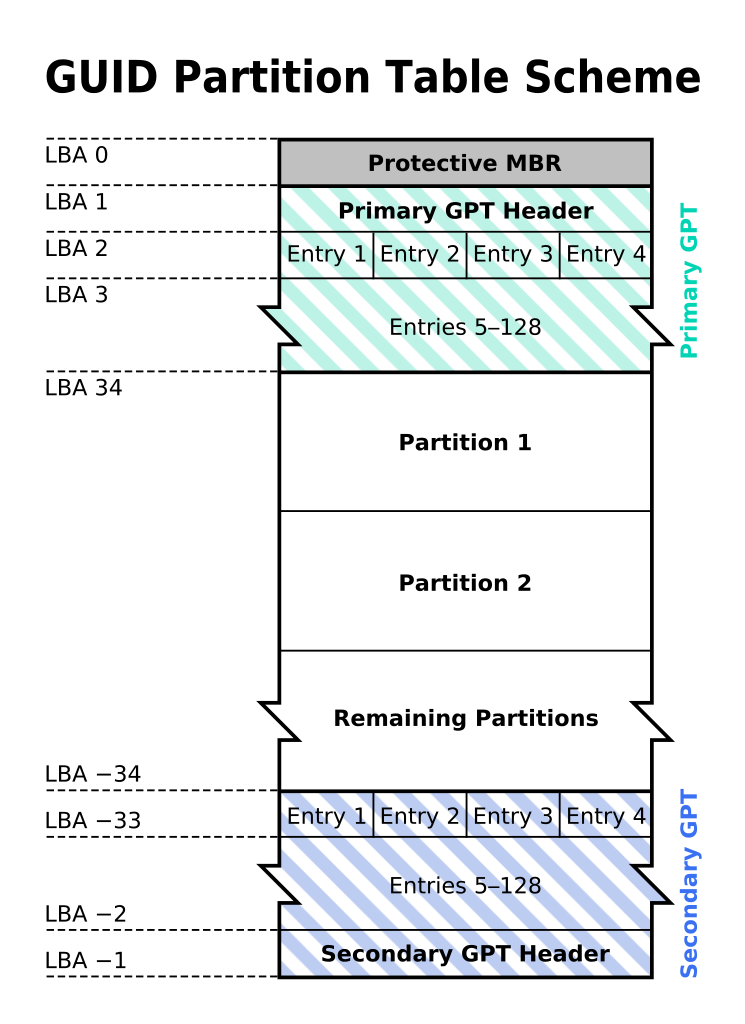
\includegraphics[scale=0.23,angle=270]{images/gpt.png}
        \captionsetup{labelformat=empty,labelsep=none}
        \transparent{0.4}%
    \end{figure}
\end{frame}


\begin{frame}[fragile]
  \frametitle{5.8 Exercise: Investigate disk with  strange PT}
    \begin{itemize}
        \item Fix the first partition table entry! \texttt{mmls mbr\_ex.raw}
    \end{itemize}
  \begin{lstlisting}[basicstyle=\tiny]
        Slot      Start        End          Length       Description
000:  Meta      0000000000   0000000000   0000000001   Primary Table (#0)
001:  -------   0000000000   0000002049   0000002050   Unallocated
002:  000:000   0000002050   0000067585   0000065536   Win95 FAT32 (0x0c)
003:  000:001   0000067586   0000133119   0000065534   Win95 FAT32 (0x0c)
004:  000:002   0000133120   0000262142   0000129023   Win95 FAT32 (0x0c)
005:  -------   0000262143   0000262143   0000000001   Unallocated
  \end{lstlisting}
    \begin{itemize}
        \item Search for partition 1 signature
    \end{itemize}
  \begin{lstlisting}[basicstyle=\tiny]
sigfind -o 510 -l AA55 mbr_ex.raw
  \end{lstlisting}
\end{frame}


\begin{frame}[fragile]
  \frametitle{5.8 Exercise: Investigate disk with  strange PT}
    \begin{itemize}
        \item The fixed partition table:
    \end{itemize}
  \begin{lstlisting}[basicstyle=\tiny]
      Slot      Start        End          Length       Description
000:  Meta      0000000000   0000000000   0000000001   Primary Table (#0)
001:  -------   0000000000   0000002047   0000002048   Unallocated
002:  000:000   0000002048   0000067583   0000065536   Win95 FAT32 (0x0c)
003:  -------   0000067584   0000067585   0000000002   Unallocated
004:  000:001   0000067586   0000133119   0000065534   Win95 FAT32 (0x0c)
005:  000:002   0000133120   0000262142   0000129023   Win95 FAT32 (0x0c)
006:  -------   0000262143   0000262143   0000000001   Unallocated
  \end{lstlisting}
    \begin{itemize}
        \item Investigate partition 3 boundaries
    \end{itemize}
  \begin{lstlisting}[basicstyle=\tiny]
dd if=mbr_ex.raw count=2049 | xxd | less
dd if=mbr_ex.raw skip=67583 count=4 | xxd | less
dd if=mbr_ex.raw skip=262142 | xxd | less
  \end{lstlisting}
\end{frame}


\begin{frame}[fragile]
  \frametitle{5.9 VBR - Volume Boot Record - Boot Sector}
  \begin{lstlisting}[basicstyle=\tiny]
# dd if=/dev/sdc1 bs=512 count=1 skip=0 |xxd

0000000: eb58 906d 6b64 6f73 6673 0000 0208 2000  .X.mkdosfs.... .     # 0xeb 0x58 0x90
0000010: 0200 0000 00f8 0000 3e00 f800 0000 0000  ........>.......     # JMP  2+88 NOP
0000030: 0100 0600 0000 0000 0000 0000 0000 0000  ................
0000040: 0000 29a2 20e9 9c46 4154 2020 2020 2020  ..). ..FAT      
0000050: 2020 4641 5433 3220 2020 0e1f be77 7cac    FAT32   ...w|.
0000060: 22c0 740b 56b4 0ebb 0700 cd10 5eeb f032  ".t.V.......^..2
...
...
00001f0: 0000 0000 0000 0000 0000 0000 0000 55aa  ..............U.


0 - 2           Size:  3    Jump to bootstrap code
3 - 10          Size:  8    OEM-ID: mkdosfs
11 - 12         Size:  2    Bytes per sector: 0x0002 -> 0x0200 (little endian)-> 512
13 (0xD)        Size:  1    Sectors per cluster: 0x08 -> 4096 bytes per cluster
50 (0x32) - 51  Size:  2    Boot sector backup: 0x0600 -> 0x0006 -> at sector 6
67 (0x43) - 70  Size:  4    Volume serial number: 0xa220e99c -> 0x9ce920a2
71 (0x47)       Size: 11    Volume label: FAT
82 (0x52)       Size:  8    Partition type: FAT32
90 (0x5A)- 509 (0x1FD)	    Bootstrap code
510 (0x1FE)     Size:  2    Signature: 0x55AA
  \end{lstlisting}
    \begin{itemize}
        \item Demo: Sleuthkit tools: \texttt{mmstat, mmls, fsstat}
    \end{itemize}
\end{frame}









\include{f06_fls}
\include{f07_car}
\include{f08_fil}
% DO NOT COMPILE THIS FILE DIRECTLY!
% This is included by the other .tex files.


\begin{frame}
    
\includegraphics[scale=0.3]{images/logo-circl-Forensics.png}
    \begin{itemize}
        \item[]
        \item[]
        \item[] 9. String Search
    \end{itemize}
\end{frame}


\begin{frame}[fragile]
  \frametitle{9.1 What is 'String Search'?}
    \begin{itemize}
       \item Search the disk image for known words
            \begin{itemize}
                \item Terms used in a secret document
                \item IBAN ot other banking details
                \item Email addresses or URLs
                \item File names or shell commands
		\item[]
            \end{itemize}
       \item Search thrue all the blocks
            \begin{itemize}
                \item Allocated blocks
                \item File slack
                \item Non allocated blocks
                \item Outside the partition borders
		\item[]
            \end{itemize}
       \item Goal
            \begin{itemize}
                \item Proof that the data was there once
                \item May even recover deleted files
                \item Identify intresting data that are close
            \end{itemize}
    \end{itemize}
\end{frame}


\begin{frame}[fragile]
  \frametitle{9.2 Steps to do a String Search}
    \begin{enumerate}
       \item Identify block/cluster size
            \begin{itemize}
		\item[] \texttt{mmls, fsstat}
            \end{itemize}
       \item Search for the string and the offset
            \begin{itemize}
		\item[] \texttt{blkls | srch\_strings | grep }
            \end{itemize}
       \item Calculate block/cluster of the string
	    \begin{itemize}
		\item[] \texttt{xxxxxxxxxx / 4096 = yyyy}
            \end{itemize}
       \item Review block/cluster content
	    \begin{itemize}
		\item[] \texttt{blkcat}
            \end{itemize}
       \item Identify inode of the block/cluster
	    \begin{itemize}
		\item[] \texttt{ifind}
            \end{itemize}
       \item Identify associated file
	    \begin{itemize}
		\item[] \texttt{ffind}
            \end{itemize}
       \item Recover file
	    \begin{itemize}
		\item[] \texttt{icat}
		\item[] Or mount and copy file
            \end{itemize}
    \end{enumerate}
\end{frame}


\newcounter{saveenumi}
\newcommand{\seti}{\setcounter{saveenumi}{\value{enumi}}}
\newcommand{\conti}{\setcounter{enumi}{\value{saveenumi}}}
\resetcounteronoverlays{saveenumi}

\begin{frame}[fragile]
  \frametitle{9.3 Exercise: What about Paulas cat?}
    \begin{enumerate}
        \item Identify cluster size
        \begin{lstlisting}[basicstyle=\tiny]
mmls circl-dfir.dd

    1      Slot      Start        End          Length       Description
 000:  Meta      0000000000   0000000000   0000000001   Primary Table (#0)
 001:  -------   0000000000   0000002047   0000002048   Unallocated
 002:  000:000   0000002048   0004917247   0004915200   NTFS / exFAT (0x07)



fsstat -o 2048 circl-dfir.dd

     File System Type: NTFS
     Volume Serial Number: 7B6E5F9427919882
     OEM Name: NTFS    
     Volume Name: CIRCL-DFIR
     Version: Windows XP

     .....

     Sector Size: 512
     Cluster Size: 4096
     Total Cluster Range: 0 - 614398
     Total Sector Range: 0 - 4915198
        \end{lstlisting}
    \seti
    \end{enumerate}
\end{frame}


\begin{frame}[fragile]
  \frametitle{9.3 Exercise: What about Paulas cat?}
    \begin{enumerate}
        \conti
        \item Search for the string \texttt{'Paula'}
        \begin{lstlisting}[basicstyle=\tiny]
blkls -e -o 2048 circl-dfir.dd | strings -a -td | grep -i paula

     157342 Paula's cat is fat.........
     157370 Paula's cat is fat.........
     .....
     157510 Paula's cat is fat.........
     157538 Paula's cat is fat.........
        \end{lstlisting}

        \item Calculate cluster of the string
        \begin{lstlisting}[basicstyle=\tiny]
echo $((157342/4096))
     38

echo $((157538/4096))
     38
        \end{lstlisting}

        \item Review cluster content
        \begin{lstlisting}[basicstyle=\tiny]
blkcat -o 2048 circl-dfir2dd 38 | strings
     .....
     Paula's cat is fat.........
     Paula's cat is fat.........
     Paula's cat is fat.........
     .....
        \end{lstlisting}
    \seti
    \end{enumerate}
\end{frame}


\begin{frame}[fragile]
  \frametitle{9.3 Exercise: What about Paulas cat?}
    \begin{enumerate}
        \conti
        \item Identify inode of the cluster
        \begin{lstlisting}[basicstyle=\tiny]
ifind -o 2048 -d 38 circl-dfir.dd 
  0-128-1
        \end{lstlisting}

        \item Identify associated file
        \begin{lstlisting}[basicstyle=\tiny]
ffind -o 2048 circl-dfir.dd 0-128-1
  //$MFT
        \end{lstlisting}

        \item Recover file
        \begin{lstlisting}[basicstyle=\tiny]
icat -o 2048 circl-dfir.dd 0-128-1 > MFT
        \end{lstlisting}
    \end{enumerate}
    \begin{itemize}
        \item[] Exercise: Manual approach - Learn from errors
        \begin{lstlisting}[basicstyle=\tiny]
dd if=circl-dfir.dd bs=4096 skip=38 count=1 | xxd | less
dd if=circl-dfir.dd bs=4096 skip=$((2048 + 38)) count=1 | xxd | less
dd if=circl-dfir.dd bs=4096 skip=$((2048/8 + 38)) count=1 | xxd | less
        \end{lstlisting}
        \end{itemize}
\end{frame}




\include{f11_reg}
% DO NOT COMPILE THIS FILE DIRECTLY!
% This is included by the other .tex files.


\begin{frame}
    
\includegraphics[scale=0.3]{images/logo-circl-Forensics.png}
    \begin{itemize}
        \item[]
        \item[]
        \item[] 12. Memory Forensics
    \end{itemize}
\end{frame}


\begin{frame}
  \frametitle{12.1 About Memory Forensics}
    \begin{itemize}
        \item Information expected
            \begin{itemize}
                \item Network connections
		\item Processes (hidden)
		\item Services (listening)
                \item Malware
                \item Registry content
                \item DLL analysis
                \item Passwords in clear text
            \end{itemize}
        \item History
            \begin{itemize}
                \item 2005: String search
		\item $\to$ EProcess structures
            \end{itemize}
        \item Finding EProcess structures
            \begin{itemize}
		\item Find the doubly linked list (ntoskrnl.exe)
		\item Brute Force searching
            \end{itemize}
    \end{itemize}
\end{frame}


\begin{frame}
  \frametitle{12.2 Get your memory dump}
    \begin{itemize}
        \item Page file, swap area: \texttt{pagefile.sys}
        \item Memory dump
            \begin{itemize}
		    \item[] \url{http://www.msuiche.net}
		    \item[] \texttt{DumpIt.exe}
                    \item[] 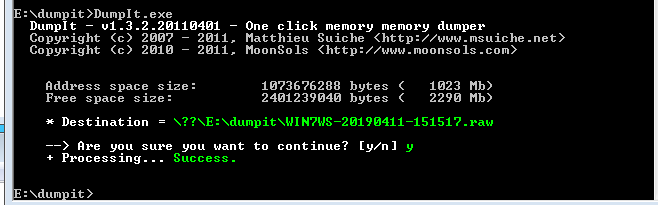
\includegraphics[scale=0.5]{images/f12_dumpit.png}
		    \item[] 
            \end{itemize}
        \item Hibernation file: \texttt{hiberfil.sys}
            \begin{itemize}
		    \item[] \texttt{powercfg /h[ibernate] [on|off]}
		    \item[] \texttt{psshutdown -h}
            \end{itemize}
    \end{itemize}
\end{frame}


\begin{frame}
  \frametitle{12.2 DumpIt}
  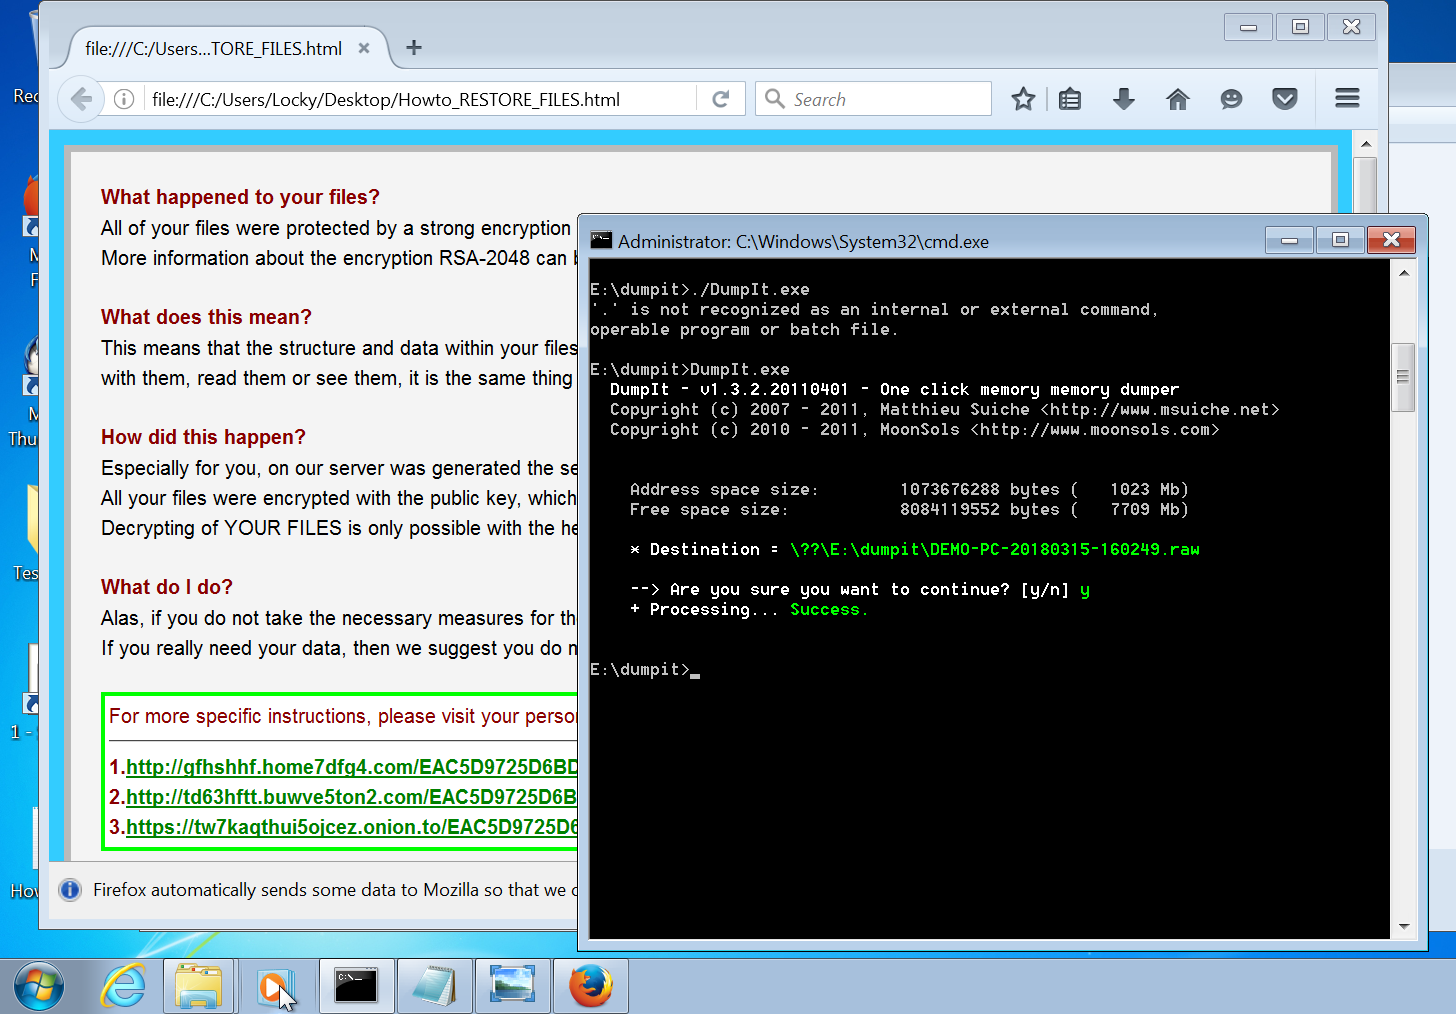
\includegraphics[scale=0.2]{images/f11_memdump.png}
\end{frame}

\begin{frame}
  \frametitle{12.3 Mandiant Redline - Malware Risk Index}
  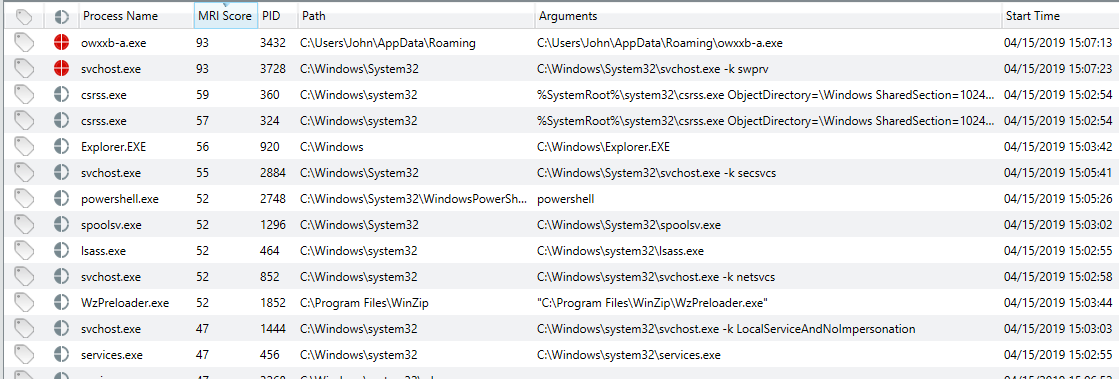
\includegraphics[scale=0.38]{images/f12_redline-1.png}
\end{frame}

\begin{frame}
  \frametitle{12.3 Mandiant Redline - Malware Risk Index}
  \begin{figure}
    \begin{center}
      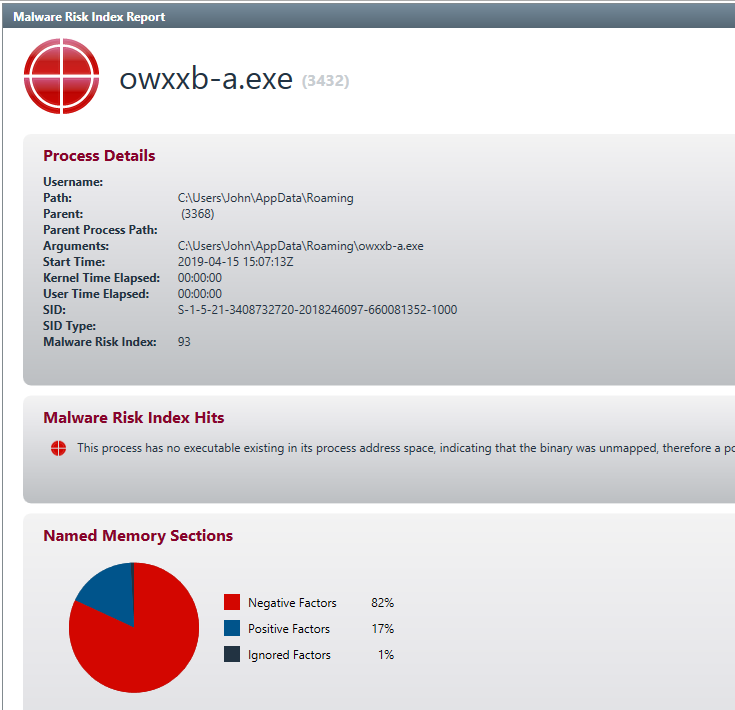
\includegraphics[scale=0.28]{images/f12_redline-2.png}

      \vspace{0.2cm}

      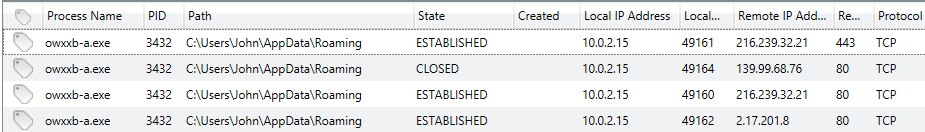
\includegraphics[scale=0.35]{images/f12_redline-3.png}
    \end{center}
  \end{figure}
\end{frame}

\begin{frame}
  \frametitle{12.3 Mandiant Redline - Malware Risk Index}
  \begin{figure}
    \begin{center}
      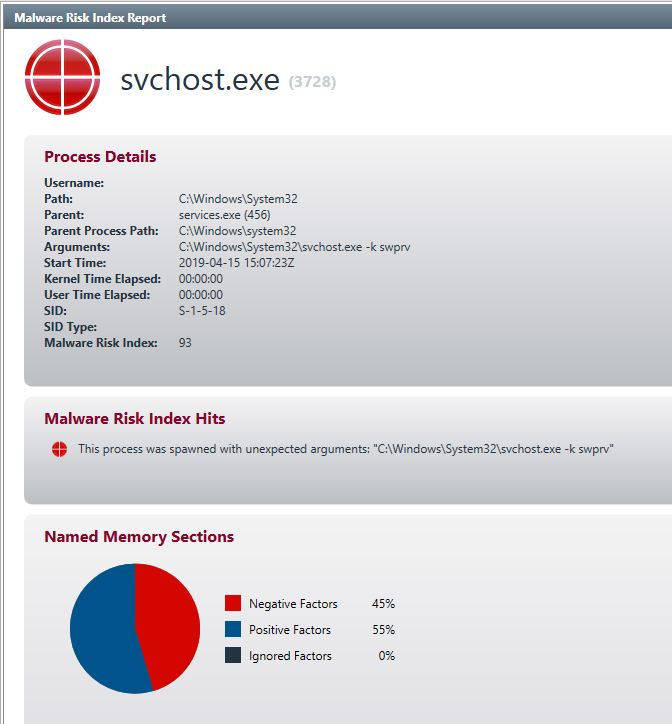
\includegraphics[scale=0.35]{images/f12_redline-4.png}
    \end{center}
  \end{figure}
\end{frame}

\begin{frame}
  \frametitle{12.3 Mandiant Redline - Hierarchical}
  \begin{figure}
    \begin{center}
      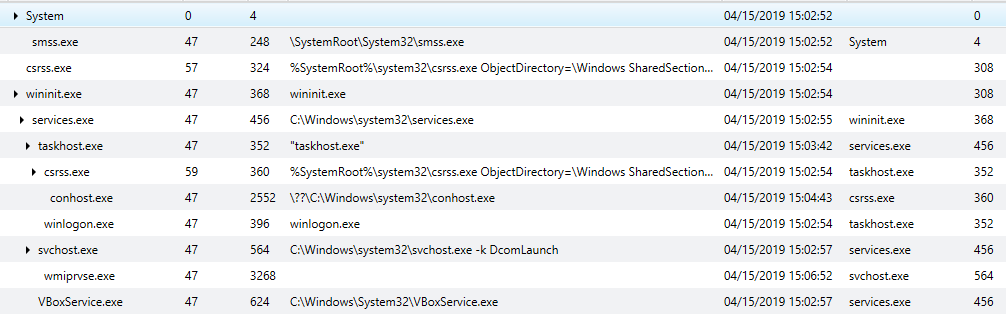
\includegraphics[scale=0.42]{images/f12_redline-5.png}

      \vspace{0.2cm}

      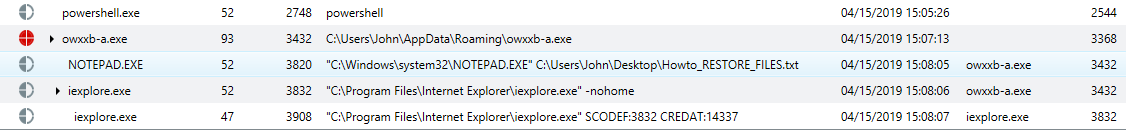
\includegraphics[scale=0.4]{images/f12_redline-7.png}
    \end{center}
  \end{figure}
\end{frame}

\begin{frame}
  \frametitle{12.3 Mandiant Redline - Timeline}
  \begin{figure}
    \begin{center}
      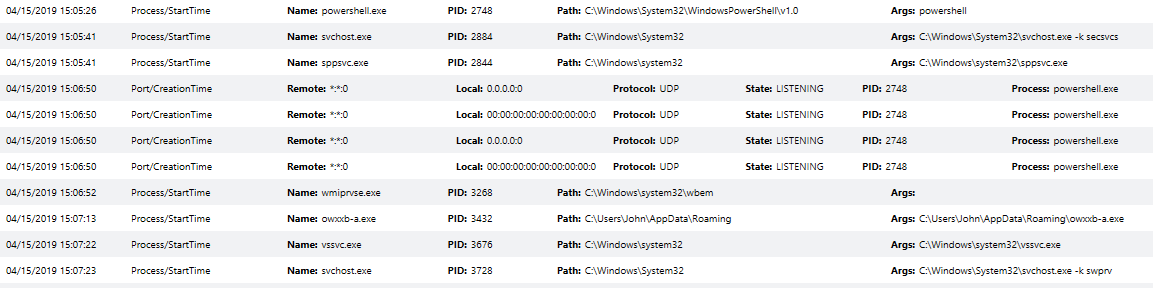
\includegraphics[scale=0.37]{images/f12_redline-6.png}

      \vspace{0.2cm}

      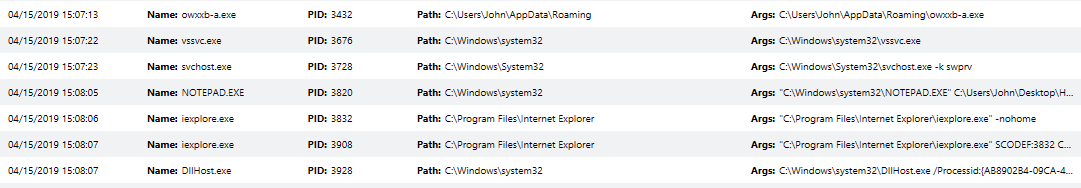
\includegraphics[scale=0.4]{images/f12_redline-8.png}
    \end{center}
  \end{figure}
\end{frame}


\begin{frame}[fragile]
  \frametitle{12.4 Volatility: Overview}
    \begin{itemize}
        \item[]
            \begin{itemize}
                \item[] \texttt{volatility -h}
                \begin{lstlisting}[basicstyle=\tiny]
...
imagecopy      	Copies a physical address space out as a raw DD image
imageinfo      	Identify information for the image
...
pslist         	Print all running processes by following the EPROCESS lists 
psscan         	Scan Physical memory for _EPROCESS pool allocations
pstree         	Print process list as a tree
psxview        	Find hidden processes with various process listings
...
sockets        	Print list of open sockets
sockscan       	Scan Physical memory for _ADDRESS_OBJECT objects (tcp sockets)
...
                \end{lstlisting}
                \item[] \texttt{volatility -f [filename] [plugin] [options]}
                \item[]
                \item[] \texttt{volatility -f DEMO-PC-20180315.raw imageinfo}
                \item[]
            \end{itemize}
    \end{itemize}
\end{frame}


\begin{frame}[fragile]
  \frametitle{12.4 Volatility: Overview}
    \begin{itemize}
        \item[]
            \begin{itemize}
                \item[] \texttt{volatility -f Win-Enc-20190415.raw imageinfo}
                \item[]
                \begin{lstlisting}[basicstyle=\tiny]
Volatility Foundation Volatility Framework 2.6
INFO    : volatility.debug    : Determining profile based on KDBG search...

          Suggested Profile(s) : Win7SP1x86_23418, Win7SP0x86, Win7SP1x86
                     AS Layer1 : IA32PagedMemory (Kernel AS)
                     AS Layer2 : FileAddressSpace
                      PAE type : No PAE
                           DTB : 0x185000L
                          KDBG : 0x82968c28L
          Number of Processors : 1
     Image Type (Service Pack) : 1
                KPCR for CPU 0 : 0x82969c00L
             KUSER_SHARED_DATA : 0xffdf0000L
           Image date and time : 2019-04-15 15:08:11 UTC+0000
     Image local date and time : 2019-04-15 17:08:11 +0200
		\end{lstlisting}
                \item[]
                \item[] \texttt{volatility --profile=Win7SP1x86 -f [filename] [plugin] [options]}
                \item[]
            \end{itemize}
    \end{itemize}
\end{frame}


\begin{frame}[fragile]
  \frametitle{12.5 Volatility: Process Analysis}
    \begin{itemize}
        \item[] \texttt{pslist}
            \begin{itemize}
                \item Running processes
                \item Process IP - PID
                \item Parent PIP - PPID
                \item Start time
            \end{itemize}
        \item[] \texttt{pstree}
            \begin{itemize}
                \item Like \texttt{pslist}
                \item Visual child-parent relation
            \end{itemize}
        \item[] \texttt{psscan}
            \begin{itemize}
                \item Brute Force
                \item Find inactive and/or hidden processes
            \end{itemize}
        \item[] \texttt{psxview}
            \begin{itemize}
                \item Run and compare some tests
                \item Correlate \texttt{psscan} and \texttt{pslist}
            \end{itemize}
    \end{itemize}
\end{frame}


\begin{frame}[fragile]
  \frametitle{12.5 Volatility: Process Analysis}
    \texttt{\footnotesize volatility --profile=Win7SP1x86 -f Win-Enc-20190415.raw pslist}
    \begin{lstlisting}[basicstyle=\tiny]
Offset(V)  Name             PID   PPID Thds  Hnds Ses Wow64 Start          
---------- ------------- ------ ------ ---- ----- --- -------------------------
0x84233af0 System             4      0   70   505 ---    0 2019-04-15 15:02:52 UTC+0000 
0x848d8288 smss.exe         248      4    2    29 ---    0 2019-04-15 15:02:52 UTC+0000
0x8487a700 csrss.exe        324    308    9   384   0    0 2019-04-15 15:02:54 UTC+0000
0x84fbb530 csrss.exe        360    352    7   274   1    0 2019-04-15 15:02:54 UTC+0000
0x84fc3530 wininit.exe      368    308    3    77   0    0 2019-04-15 15:02:54 UTC+0000
0x84fd0530 winlogon.exe     396    352    4   112   1    0 2019-04-15 15:02:54 UTC+0000
0x85048a18 services.exe     456    368    8   203   0    0 2019-04-15 15:02:55 UTC+0000
0x8505ac00 lsass.exe        464    368    7   580   0    0 2019-04-15 15:02:55 UTC+0000
0x8505caa0 lsm.exe          472    368   10   145   0    0 2019-04-15 15:02:55 UTC+0000
...
...
...
0x85050b60 WmiPrvSE.exe    3268    564    9   175   0    0 2019-04-15 15:06:52 UTC+0000
0x8438bd40 owxxb-a.exe     3432   3368   15   471   1    0 2019-04-15 15:07:13 UTC+0000
0x84394030 VSSVC.exe       3676    456    6   123   0    0 2019-04-15 15:07:22 UTC+0000
0x84394488 svchost.exe     3728    456    6    70   0    0 2019-04-15 15:07:23 UTC+0000
0x84a243c8 notepad.exe     3820   3432    1    64   1    0 2019-04-15 15:08:05 UTC+0000
0x846d8030 iexplore.exe    3832   3432   19   427   1    0 2019-04-15 15:08:06 UTC+0000
0x846d2d40 iexplore.exe    3908   3832   11   293   1    0 2019-04-15 15:08:07 UTC+0000
0x846e5a58 dllhost.exe     3928    564    6    94   1    0 2019-04-15 15:08:07 UTC+0000
0x84684d40 dllhost.exe     4012    564   10   212   1    0 2019-04-15 15:08:08 UTC+0000
    \end{lstlisting}
\end{frame}


\begin{frame}[fragile]
  \frametitle{12.5 Volatility: Process Analysis}
    \texttt{\footnotesize volatility --profile=Win7SP1x86 -f Win-Enc-20190415.raw pslist}
    \begin{lstlisting}[basicstyle=\tiny]
Offset(P)  Name          PID pslist psscan thrdproc pspcid csrss session deskthrd
---------- ---------- ------ ------ ------ -------- ------ ----- ------- --------
.....
.....
0x3f60f030 taskhost.exe     352 True   True   True     True   True  True    True
0x3fa84d40 dllhost.exe     4012 True   True   True     True   True  True    True
0x3ec23148 spoolsv.exe     1296 True   True   True     True   True  True    True
0x3f63f470 explorer.exe     920 True   True   True     True   True  True    True
0x3ff0bd40 owxxb-a.exe     3432 True   True   True     True   True  True    True
0x3f3d0530 winlogon.exe     396 True   True   True     True   True  True    True
0x3f3c3530 wininit.exe      368 True   True   True     True   True  True    True
0x3ec9f030 svchost.exe      688 True   True   True     True   True  True    True
0x3ef3d758 VBoxTray.exe    1832 True   True   True     True   True  True    True
0x3fae5a58 dllhost.exe     3928 True   True   True     True   True  True    True
0x3ec50b60 WmiPrvSE.exe    3268 True   True   True     True   True  True    True
0x3ec88b90 svchost.exe      564 True   True   True     True   True  True    True
0x3ecd3768 svchost.exe      820 True   True   True     True   True  True    True
0x3ef4f030 SearchIndexer.  2008 True   True   True     True   True  True    True
0x3ec08d40 svchost.exe     1444 True   True   True     True   True  True    True
0x3ed10d40 svchost.exe     1008 True   True   True     True   True  True    True
0x3f6243c8 notepad.exe     3820 True   True   True     True   True  True    True
0x3ecd95f8 svchost.exe      852 True   True   True     True   True  True    True
0x3fad2d40 iexplore.exe    3908 True   True   True     True   True  True    True
.....
.....
    \end{lstlisting}
\end{frame}


\begin{frame}[fragile]
  \frametitle{12.6 Volatility: Network Analysis}
    \begin{itemize}
        \item Windows XP and 2003 Server
            \begin{itemize}
                \item \texttt{connections}
                \item \texttt{connscan}
                \item \texttt{sockets}
            \end{itemize}
        \item Windwos 7
            \begin{itemize}
                \item \texttt{netscan}
            \end{itemize}
    \end{itemize}
    \texttt{\footnotesize volatility --profile=Win7SP1x86 -f Win-Enc-20190415.raw netscan}
    \begin{lstlisting}[basicstyle=\tiny]
Proto   Local Address       Foreign Address     State           Pid     Owner
.....
UDPv4   0.0.0.0:0           *:*                                2748     powershell.exe 
UDPv6   :::0                *:*                                2748     powershell.exe
TCPv4   0.0.0.0:49155       0.0.0.0:0           LISTENING       456     services.exe
TCPv4   0.0.0.0:49156       0.0.0.0:0           LISTENING       464     lsass.exe
TCPv6   :::49156            :::0                LISTENING       464     lsass.exe
TCPv4   10.0.2.15:49167     2.17.201.11:80      ESTABLISHED    1128     svchost.exe
TCPv4   10.0.2.15:49166     93.184.220.29:80    ESTABLISHED    1128     svchost.exe
TCPv4   10.0.2.15:49165     50.62.124.1:80      ESTABLISHED    3432     owxxb-a.exe
TCPv4   10.0.2.15:49160     216.239.32.21:80    ESTABLISHED    3432     owxxb-a.exe
TCPv4   10.0.2.15:49162     2.17.201.8:80       ESTABLISHED    3432     owxxb-a.exe
TCPv4   10.0.2.15:49168     13.107.21.200:80    ESTABLISHED    3832     iexplore.exe
TCPv4   10.0.2.15:49159     94.23.7.52:80       CLOSE_WAIT     2748     powershell.exe
.....
    \end{lstlisting}
\end{frame}


\begin{frame}[fragile]
  \frametitle{12.7 Volatility: Exercise}
      \texttt{\footnotesize volatility --profile=Win7SP1x86 -f Win-Enc-20190415.raw malfind}
      \begin{lstlisting}[basicstyle=\tiny]
Process: owxxb-a.exe Pid: 3432 Address: 0x400000
Vad Tag: VadS Protection: PAGE_EXECUTE_READWRITE
Flags: CommitCharge: 134, MemCommit: 1, PrivateMemory: 1, Protection: 6

0x00400000  4d 5a 90 00 03 00 00 00 04 00 00 00 ff ff 00 00   MZ..............
0x00400010  b8 00 00 00 00 00 00 00 40 00 00 00 00 00 00 00   ........@.......
0x00400020  00 00 00 00 00 00 00 00 00 00 00 00 00 00 00 00   ................
0x00400030  00 00 00 00 00 00 00 00 00 00 00 00 08 01 00 00   ................

0x00400000 4d               DEC EBP
0x00400001 5a               POP EDX
0x00400002 90               NOP

      \end{lstlisting}
      \texttt{\footnotesize volatility --profile=Win7SP1x86 -f Win-Enc-20190415.raw getsids}
      \begin{lstlisting}[basicstyle=\tiny]
powershell.exe (2748): S-1-5-21-3408732720-2018246097-660081352-1000 (John)
owxxb-a.exe (3432): S-1-5-21-3408732720-2018246097-660081352-1000 (John)
notepad.exe (3820): S-1-5-21-3408732720-2018246097-660081352-1000 (John)
iexplore.exe (3832): S-1-5-21-3408732720-2018246097-660081352-1000 (John)
iexplore.exe (3908): S-1-5-21-3408732720-2018246097-660081352-1000 (John)
dllhost.exe (3928): S-1-5-21-3408732720-2018246097-660081352-1000 (John)

      \end{lstlisting}
	\footnotesize{Create memdump of malicious process and search for suspicious URLs!}
\end{frame}








\include{f13_out}

\end{document}

